% Near: technical and business report
% Build: pdflatex near_report && pdflatex near_report   (twice, for the table of contents)
% Illustrations: each \nanofig shows its Nano Banana prompt until figures/<name>.png exists,
% then the image replaces the prompt box automatically. All prompts: figure_prompts.md
\documentclass[11pt,a4paper]{report}

\usepackage[utf8]{inputenc}
\usepackage[T1]{fontenc}
\usepackage{lmodern}
\usepackage[english]{babel}
\usepackage[a4paper,margin=2.3cm,headheight=14pt]{geometry}
\usepackage{microtype}
\usepackage{amsmath,amssymb}
\usepackage{graphicx}
\usepackage[table]{xcolor}
\usepackage{booktabs,tabularx,longtable,multirow,array}
\usepackage{siunitx}
\usepackage{enumitem}
\usepackage{caption}
\usepackage{float}
\usepackage{listings}
\usepackage[most]{tcolorbox}
\usepackage{pgfplots}
\usepackage{fancyhdr}
\usepackage{titlesec}
\usepackage[hidelinks]{hyperref}
\pgfplotsset{compat=1.17}
% Unicode characters used in the prompts and tables (pdflatex)
\DeclareUnicodeCharacter{2192}{\ensuremath{\rightarrow}}
\DeclareUnicodeCharacter{2190}{\ensuremath{\leftarrow}}
\DeclareUnicodeCharacter{2194}{\ensuremath{\leftrightarrow}}
\DeclareUnicodeCharacter{03C3}{\ensuremath{\sigma}}
\DeclareUnicodeCharacter{03B8}{\ensuremath{\theta}}
\DeclareUnicodeCharacter{03B2}{\ensuremath{\beta}}
\DeclareUnicodeCharacter{2248}{\ensuremath{\approx}}
\DeclareUnicodeCharacter{00D7}{\ensuremath{\times}}
\DeclareUnicodeCharacter{2264}{\ensuremath{\leq}}
\DeclareUnicodeCharacter{2265}{\ensuremath{\geq}}
\DeclareUnicodeCharacter{2713}{\ensuremath{\checkmark}}
\DeclareUnicodeCharacter{2212}{\ensuremath{-}}
\DeclareUnicodeCharacter{2011}{-}
\sisetup{group-separator={,},detect-all}

% ---------------------------------------------------------------- colours
\definecolor{navy}{HTML}{0D1110}
\definecolor{cyanN}{HTML}{1AA7C4}
\definecolor{amberN}{HTML}{E09A2B}
\definecolor{redN}{HTML}{E5484D}
\definecolor{greenN}{HTML}{3FA877}
\definecolor{greyN}{HTML}{8B9A94}
\definecolor{promptbg}{HTML}{F3F7F8}
\definecolor{promptframe}{HTML}{1AA7C4}

% ---------------------------------------------------------------- layout
\setlist{itemsep=2pt,topsep=4pt}
\captionsetup{font=small,labelfont=bf}
\titleformat{\chapter}[display]{\normalfont\bfseries\color{navy}}{\large\color{cyanN}Chapter \thechapter}{4pt}{\Huge}
\titlespacing*{\chapter}{0pt}{-10pt}{18pt}
\pagestyle{fancy}
\fancyhf{}
\fancyhead[L]{\small\color{greyN}Near}
\fancyhead[R]{\small\color{greyN}\nouppercase{\leftmark}}
\fancyfoot[C]{\small\thepage}
\renewcommand{\headrulewidth}{0.3pt}

\lstset{basicstyle=\ttfamily\footnotesize,breaklines=true,frame=single,rulecolor=\color{greyN!50},
        backgroundcolor=\color{promptbg},columns=fullflexible,keepspaces=true}

% ---------------------------------------------------------------- figures
% \nanofig[width]{file name, no extension}{caption}{Nano Banana prompt}
\newcommand{\nanofig}[4][0.92\linewidth]{%
  \begin{figure}[htbp]\centering
  \IfFileExists{figures/#2.png}{\includegraphics[width=#1,height=0.42\textheight,keepaspectratio]{figures/#2.png}}{%
    \begin{tcolorbox}[enhanced,colback=promptbg,colframe=promptframe,width=#1,arc=2mm,
      boxrule=0.6pt,fonttitle=\small\bfseries,
      title={Illustration to generate \hfill \texttt{figures/#2.png}}]
      \footnotesize\textbf{Nano Banana prompt.} #4
  \end{tcolorbox}}
  \caption{#3}\label{fig:#2}
  \end{figure}}

% boxes for honest caveats and key results
\newtcolorbox{caveat}[1][What this does not show]{colback=amberN!6,colframe=amberN,
  fonttitle=\small\bfseries,title={#1},arc=1.5mm,boxrule=0.5pt}
\newtcolorbox{keyresult}[1][Measured]{colback=cyanN!6,colframe=cyanN,
  fonttitle=\small\bfseries,title={#1},arc=1.5mm,boxrule=0.5pt}

\newcommand{\code}[1]{\texttt{\small #1}}

\begin{document}

% ---------------------------------------------------------------- title
\begin{titlepage}
  \centering
  \vspace*{1.2cm}
  {\color{cyanN}\large European Defence Tech Hackathon, Paris, 20--22 November 2026\par}
  \vspace{0.3cm}
  {\color{greyN}Challenge 01: Voice-to-Map, real-time positional tracking\par}
  \vspace{1.4cm}
  {\fontsize{48}{52}\selectfont\bfseries\color{navy} Near\par}
  \vspace{0.4cm}
  {\LARGE Finding the wounded when GPS is jammed\par}
  \vspace{0.3cm}
  {\large Technical and business report\par}
  \vspace{1cm}
  \IfFileExists{figures/cover.png}{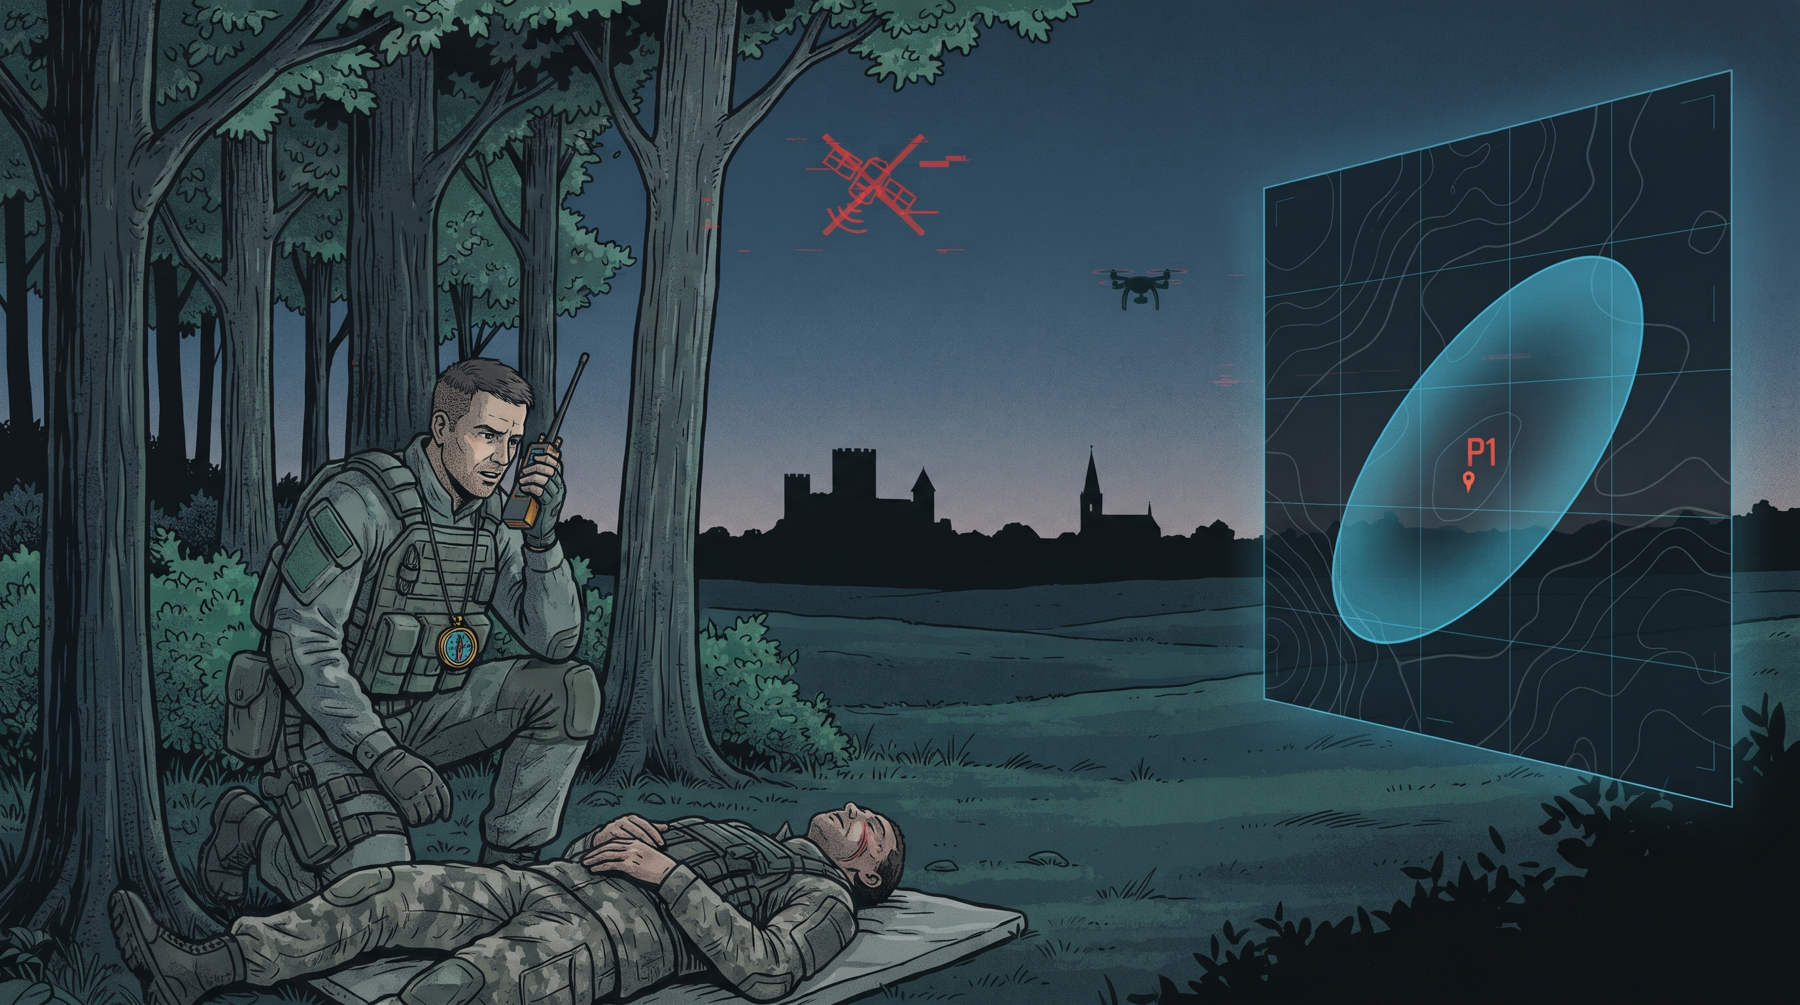
\includegraphics[width=0.85\linewidth]{figures/cover.png}}{%
  \begin{tcolorbox}[colback=promptbg,colframe=promptframe,width=0.85\linewidth,arc=2mm,
    title={\small Illustration to generate \hfill \texttt{figures/cover.png}}]
  \footnotesize\textbf{Nano Banana prompt.} Cinematic wide illustration at dusk. In the foreground a combat medic
  kneels in a tree line beside a wounded soldier, speaking into a handheld tactical radio; a small compass hangs from
  his vest. Behind them, across a field, the silhouette of a medieval castle keep and a church spire. In the sky, a
  faint red glitch overlay of a satellite icon crossed out (GPS jammed) and a distant small quadcopter drone. On the
  right third of the image, as if projected in the air, a translucent dark-blue tactical map with a cyan uncertainty
  ellipse shrinking onto a red casualty pin labelled ``P1''. Muted realistic colours, no gore, no national flags, no readable text except ``P1''. 16:9. Colour palette (use only these): navy \#0D1110, cyan \#1AA7C4, amber \#E09A2B, red \#E5484D, green \#3FA877, grey \#8B9A94, plus white for text on dark shapes.
  \end{tcolorbox}}
  \vfill
  {\large Team Fricassé: Taher Ayadi, Aziz Maatoug\par}
  \vspace{0.2cm}
  {\color{greyN}22 November 2026 \quad·\quad Code: \texttt{github.com/Taher1412/Near}\par}
\end{titlepage}

\chapter*{Executive summary}
\addcontentsline{toc}{chapter}{Executive summary}
\markboth{Executive summary}{}

Under GPS jamming, a soldier often doesn't know where he is. He can still say what he sees:
``the castle keep at my 11 o'clock, a church at bearing 240, sun at my 1 o'clock''. Near turns
that sentence into a position. When the position is still vague, it asks the one spoken question
that narrows it down most. Then it reads the answer back, and puts the casualty on the
coordinator's map with a MIST card, a tourniquet timer and a place in the evacuation order.
The name of the method is old: the \emph{problème de Pothenot} is the French surveyors' name for
finding your own position from the angles to known points.

Around eleven teams took the same hackathon challenge. All of them map what a speaker says, and
all of them assume the speaker knows where he is. We built for the case where he doesn't.

\paragraph{What Near does, end to end.}
\begin{itemize}
  \item \textbf{Locates the speaker without GPS.} A likelihood grid (25 m cells $\times$ 72 headings)
        combines spoken clock directions, compass bearings, the sun, landmarks seen or not seen
        (with a LiDAR line-of-sight model), ground clues, sounds, echoes and the noise level.
  \item \textbf{Asks back.} Candidate questions are scored by the position error and the entropy they
        are expected to remove. Fewer and easier questions are asked when the voice sounds stressed.
  \item \textbf{Organises the casualty.} MIST card, MARCH state, ``worse in'' countdowns, mobility,
        an impact graph from wound to kit, team size, a 3D body twin and an optional heart rate
        from a chest recording. All of this is decision support only.
  \item \textbf{Maps threats.} Drones, gunfire and explosions are heard by the microphone, or named
        by voice, and drawn as zones; overlapping reports from several units mark the likely
        source area.
  \item \textbf{Brings people back.} A casualty who can walk is guided to the collection point along
        the safest walking route, with spoken landmark-based legs and a pin that moves by dead
        reckoning. A casualty who can't walk gets a medic route instead.
  \item \textbf{Works in war conditions.} With no internet, no GPS and no phone network, everything
        runs on one laptop: local Whisper speech-to-text, a local Mistral 7B, offline map tiles,
        offline voices. The laptop listens to the tactical voice radio, routes each message by
        callsign and answers on the radio. A phone, if the unit has one, runs a 5.5M-parameter
        sound model offline and sends its measurements as ~2 s of audio tones through the same
        radio.
\end{itemize}

\paragraph{Key numbers (all measured; methods in Chapter~\ref{ch:eval}).}
\begin{itemize}
  \item Spots where at least two landmarks are truly visible, ask-back loop with up to three
        questions: median error \textbf{43 m}.
  \item Spoken compass bearings to two named landmarks: median error \textbf{71 m}, against
        250 m with clock directions.
  \item Aim \& tap (phone tilt and turn): median error \textbf{75 m} in the streets where a landmark
        top is in sight, against 417 m before the 3D model.
  \item Drones heard through a simulated radio: \textbf{100 \%} detected by our radio-trained
        5.5M-parameter model, against 6--9 \% for the 86M-parameter drone detector it learned from.
  \item Data packets through a simulated lossy digital radio: \textbf{39/40} delivered with
        two-copy combining, against 10/40 with one copy.
  \item Safest route on the city's walking network: about 30 ms. In the test scene, a 390 m detour
        avoided 398 m inside a small-arms zone.
\end{itemize}

\paragraph{Business.} Near is software. It runs on a laptop and radios the units already own, and
it needs no new hardware in the field. The first customers are military medical services and
command posts in Europe and Ukraine, where GPS interference is routine and drones have made the
``golden hour'' unreachable. The same engine fits civilian rescue: lost callers who can't give
an address, mountain rescue, and disaster zones without a network. Chapter~\ref{ch:business}
covers the market, the competition, the business model and the risks.

\paragraph{What is not proven yet.} Every result above comes from real map data and real recordings, but the soldier,
the radio channel or both are simulated. Before anyone relies on Near, it needs one walk by the
Château de Vincennes with GPS off, recordings through the unit's real radio, and medical
validation of every threshold. Chapter~\ref{ch:roadmap} lists these tests.

\tableofcontents
\listoffigures
\listoftables

\chapter{The problem}\label{ch:problem}

\section{Casualty reporting assumes a known position}

Every casualty report format in use starts with a location. The NATO 9-line MEDEVAC request
puts it on line 1. Tactical apps and battle management systems take it from the device's GPS.
The challenge brief we answered (Voice-to-Map, sponsor Lysk) asks for spoken position updates
turned into map updates, and suggests OpenStreetMap geocoding plus an LLM for intent
extraction. Every team we saw built that pipeline: speech, then text, then a place name, then a
pin.

All of it fails in the same situation: the person reporting doesn't know where he is.

\section{GPS is jammed, and not only at the front}

Satellite navigation is now routinely denied or falsified over large areas, not only on the
front line. Governments around the Baltic reported to ICAO that about 123,000 flights were
affected by GPS interference between January and April 2025, with authorities in Estonia saying
85 \% of flights there were affected \cite{gps123k,trtgps}. Poland recorded 2,732 jamming and
spoofing cases in January 2025 alone \cite{trtgps}. A receiver under spoofing is worse than a
receiver with no fix: it shows a confident, wrong position.

On the ground, the soldier near the front knows roughly which sector he's in and can see what
is around him. He usually can't produce a grid reference under fire, at night or while treating
a wounded friend.

\section{Drones have removed the golden hour}

In Ukraine, persistent drone surveillance has changed how casualties are moved. A Ukrainian
officer at the NATO-Ukraine training centre said the golden hour ``does not exist'' any more, and
that only a ``golden day'' remains \cite{goldenday}. Medics report that evacuations by day are
rare. Teams wait for darkness, bad weather or smoke, and in some sectors the wounded wait in
forward positions for days \cite{wotr,daylight}. FPV drones and loitering munitions are reported
to cause up to 90 \% of casualties in some sectors \cite{dignitas}. Ground robots and drones are
now used to carry the wounded over the last few kilometres \cite{aspi}.

Three consequences shape our design:
\begin{enumerate}
  \item \textbf{Locating the casualty precisely matters more}, because the evacuation team gets one
        attempt, at night, along a route that must avoid drones.
  \item \textbf{Every transmission is a risk.} Radio emissions are located and targeted, so the
        system must get the most information from the fewest and shortest transmissions.
  \item \textbf{The wounded wait longer}, so time-critical threats (bleeding, airway, hypothermia,
        tourniquet time) need tracking for hours, not minutes.
\end{enumerate}

\nanofig{problem}{The situation Near is built for: GPS denied, drones overhead, a medic who can describe
what he sees but can't give a grid reference.}{Split-panel editorial illustration, 16:9, flat vector style
with subtle texture, plain white background, cyan, amber and red accents. Left panel titled ``GPS DENIED'':
a soldier's wrist GPS showing a glitched screen with ``NO FIX'' and a red jamming wave pattern radiating from
a distant antenna truck. Middle panel titled ``DRONES OVERHEAD'': a small quadcopter silhouette above a
tree line, a dotted red cone below it, two medics crouched under trees with a stretcher. Right panel titled
``WHERE ARE WE?'': the medic holding a radio, a speech bubble with a small castle keep icon, a church icon
and a sun icon with arrows, and a question mark over a blank map. Clean sans-serif labels, exactly these three
titles, no other text, no gore. Colour palette (use only these): navy \#0D1110, cyan \#1AA7C4, amber \#E09A2B, red \#E5484D, green \#3FA877, grey \#8B9A94, plus white for text on dark shapes.}

\section{What already exists and why it isn't enough}

\begin{table}[htbp]\centering\small
\caption{How existing approaches handle a speaker who doesn't know his position.}\label{tab:gap}
\begin{tabularx}{\linewidth}{>{\raggedright}p{3.6cm}X>{\raggedright\arraybackslash}p{3.8cm}}
\toprule
Approach & What it does & With GPS jammed and an unsure speaker\\
\midrule
Device GPS in tactical apps (ATAK-type tools, battle management systems) & Shares the position of each device & No fix, or a spoofed one\\
Other teams on this challenge (e.g. LowKey, Ground Truth, ELARIS) & Speech $\rightarrow$ place name $\rightarrow$ geocoded pin; trust scores and ageing of reports & Needs the speaker to name the place he is at\\
Voice-guided navigation (hasky labs) & Gives directions from a known position & Needs the starting position\\
Acoustic gunshot and drone sensors & Locate sources with dedicated microphone arrays & New hardware, fixed installations\\
Map reading and compass resection & The trained soldier's manual method & Slow, needs a map and calm; few do it under fire\\
\bottomrule
\end{tabularx}
\end{table}

The manual method in the last row is the one we automate. Resection from bearings to known points
is standard land-navigation doctrine, and Pothenot's problem is its classic form. Near does it
from speech, tolerates noise and missing data, and asks for the observation that would help most.

\section{Requirements we set ourselves}

\begin{itemize}
  \item No GPS, no internet, no phone network required. Any of them is used if present.
  \item No new hardware in the field. The soldier's radio is enough; a phone adds sensors.
  \item Answers in seconds: under 300 ms per position update, a few seconds per report.
  \item Honest uncertainty: every position comes with a radius and, when several areas fit, all of them.
  \item English and French, and radio procedure words (callsigns, ``over'').
  \item Medical output is decision support for trained medics: organising, timing and ordering, never diagnosing.
\end{itemize}

\chapter{The solution in one page}\label{ch:solution}

Near listens to one spoken report and keeps a running answer to three questions: where is the
casualty, how bad is it, and how do we get them out. Figure~\ref{fig:concept} shows the loop.

\nanofig{concept}{The Near loop: describe what you see, get located, answer one question, get the read-back.}
{Horizontal four-step infographic, 16:9, clean flat vector, plain white background, navy text, cyan and amber accents.
Step 1 ``DESCRIBE'': a soldier icon with a radio and a speech bubble showing a castle icon with ``11 o'clock'',
a church icon with ``240°'' and a sun icon with ``1 o'clock''. Step 2 ``LOCATE'': a top-down street map with a
large translucent cyan ellipse and two smaller dashed circles labelled A and B. Step 3 ``ASK'': a speech bubble
from a laptop saying ``Is the church left or right of the keep?'' with a small bar chart labelled ``bits gained''.
Step 4 ``READ BACK'': the ellipse shrunk to a small circle on a street corner, a red pin labelled ``P1'', a timer
``TQ 72:14'' and the text ``within 60 m''. Thin arrows between steps, a curved arrow from step 3 back to step 2.
Use exactly the quoted labels. Colour palette (use only these): navy \#0D1110, cyan \#1AA7C4, amber \#E09A2B, red \#E5484D, green \#3FA877, grey \#8B9A94, plus white for text on dark shapes.}

\section{Three users}

\paragraph{The field user} is a buddy or a medic, sometimes the casualty himself. He holds push-to-talk
and speaks a report in his own words:
\begin{quote}\itshape
``This is Bravo 2. One casualty, blast, left leg bleeding, tourniquet on at 14:32, conscious and
breathing. We're in a tree line. I see the castle keep at my 11 o'clock, a church at bearing 240,
sun at my 1 o'clock. Over.''
\end{quote}
He hears back:
\begin{quote}\itshape
``Bravo 2, this is CCP. Copy. One urgent casualty, tourniquet 14:32. Stretcher needed. Two possible
areas, best one within 300 metres. Question: if you have a compass, what is the bearing to the
castle keep? Degrees or mils. Over.''
\end{quote}
One to three exchanges later the position is confirmed, and if the casualty can walk, the read-back
turns into directions to the collection point.

\paragraph{The coordinator} sits at the casualty collection point (CCP) with a laptop. The map shows
every casualty with its uncertainty, the threat zones, the routes. Side tiles show the MIST card,
the condition with countdowns, the impact graph, the kit and team to send, and the evidence behind
the position (Figure~\ref{fig:dashboard}).

\paragraph{The radio operator} is often the coordinator. In radio mode the laptop listens to the
radio, transcribes each transmission and proposes the reply. The operator approves, edits or
skips it, and the laptop speaks it into the radio.

\nanofig{dashboard}{The coordinator dashboard: evacuation order, casualty card, map with uncertainty and threat
zones, location evidence, sound analysis, impact graph and the team to send.}
{High-fidelity dark-mode UI mockup of a tactical web dashboard, 16:9, the dashboard window itself in near-black navy tones on a plain white background,
thin 1 px borders, monospace numbers. Top bar: ``NEAR · COORDINATOR'', a red ``P1'' badge, KPI boxes
``POSITION ±60 m'', ``TOURNIQUET 72:14'' (amber), ``MOBILITY stretcher'', ``WORSE IN 4 min'' (red), buttons
``Radio'', ``Simulate''. Left column: ``EVACUATION ORDER'' list of three rows with P1, P1, P2 badges and timers.
Centre: a dark map of a small town with a castle, a cyan route line to a ``CCP'' marker, a translucent red circle
labelled ``SMALL-ARMS FIRE'', a pink dashed circle labelled ``DRONE'', a cyan ellipse around a red pin. Right
column: ``CASUALTY'' card with M A R C H rows coloured red/green/grey, ``LOCATION'' panel with a top-down building
plan and echo rings. Bottom: a left-to-right graph of boxes ``Reported → Body region → Possibly impacted → MARCH
threat → Bring''. Crisp, realistic product screenshot style. Colour palette (use only these): navy \#0D1110, cyan \#1AA7C4, amber \#E09A2B, red \#E5484D, green \#3FA877, grey \#8B9A94, plus white for text on dark shapes.}

\section{Three ways to run}

\begin{table}[htbp]\centering\small
\caption{Deployment modes. Near detects what is available and degrades gracefully.}\label{tab:modes}
\begin{tabularx}{\linewidth}{lXXX}
\toprule
& Connected & Radio only (war default) & Radio + offline phone\\
\midrule
Field equipment & Phone with a browser & Tactical voice radio & Radio + phone in airplane mode\\
Link to the CCP & Wi-Fi, 4G or a tunnel (HTTPS) & Voice channel & Voice channel carrying data tones\\
Speech-to-text & Local Whisper (or Chrome online) & Local Whisper on the laptop & Local Whisper on the laptop\\
Sensors used & Mic (sound, echoes, noise), compass, gyroscope, steps, optional last GPS fix & What is said; sounds heard through the radio & Phone measures offline, sends $\sim$30 B packets\\
Position clues & All & Clock directions, compass bearings, sun, ground, pace count & All, except the raw audio\\
Guidance & Spoken + live pin & Spoken over the radio + dead reckoning by time and pace count & On the phone: compass arrow, steps, spoken turns\\
\bottomrule
\end{tabularx}
\end{table}

\nanofig{modes}{The three deployment modes side by side.}
{Three-column technical diagram, 16:9, flat vector on white, navy lines, cyan and amber highlights. Column
``CONNECTED'': a phone icon linked by a Wi-Fi symbol to a laptop icon. Column ``RADIO ONLY'': a handheld tactical
radio linked by zig-zag radio waves to a second radio, which is linked by an audio cable to a laptop; a crossed-out
satellite icon and a crossed-out cloud icon above. Column ``RADIO + OFFLINE PHONE'': a phone held next to a radio,
small sound-wave tones drawn between the phone speaker and the radio microphone, a label ``~2 s of tones,
30 bytes'', radio waves to the laptop. Under each laptop a small map with a pin. Titles exactly ``CONNECTED'',
``RADIO ONLY'', ``RADIO + OFFLINE PHONE''. Colour palette (use only these): navy \#0D1110, cyan \#1AA7C4, amber \#E09A2B, red \#E5484D, green \#3FA877, grey \#8B9A94, plus white for text on dark shapes.}

\section{What the jury sees in the demo}

\begin{enumerate}
  \item An empty map of Vincennes on the coordinator laptop, drawn from local data with no internet.
  \item Outside by the Château, GPS off, a teammate plays the casualty; the other speaks the report on the radio.
  \item The map shows a large ellipse, sometimes two areas. The laptop asks, on the radio, the question
        that splits them.
  \item The answer comes in. The ellipse shrinks onto one street. Read-back: ``Position within 60 metres,
        priority 1''.
  \item A second unit reports a drone. A pink zone appears; the walking casualty's route bends around it.
  \item The evacuation list reorders live; the tourniquet timer keeps running.
\end{enumerate}

\chapter{System architecture}\label{ch:arch}

Near is a single Python service (FastAPI) and two web pages. All the intelligence runs on the
coordinator's laptop. The phone page and the coordinator page talk to it over HTTP and a
WebSocket. In radio mode, an audio cable takes their place.

\nanofig{architecture}{System architecture. Everything inside the laptop box runs offline.}
{Detailed software architecture diagram, 16:9, plain white background, flat vector, navy outlines, rounded boxes, cyan
for data flow, amber for audio flow. Left: three input boxes stacked: ``Field phone (browser, offline app)'',
``Tactical radio (voice + data tones)'', ``Typed text''. Centre: a large rounded box titled ``Near server (laptop,
offline)'' containing a pipeline of boxes left to right: ``Speech-to-text (Whisper)'' → ``Extraction (rules +
Mistral 7B)'' → ``Constraints'' → ``Localisation grid'' → ``Question selector'' → ``Read-back''; below it a second
row: ``Acoustic analysis (YAMNet, AST, Near-small)'', ``Casualty model (MIST, MARCH, mobility)'', ``Danger zones'',
``Routing + guidance'', ``Modem + packets''; at the bottom a wide box ``State store'' and a box ``WebSocket''.
Right: ``Coordinator map (Leaflet, offline tiles)''. Bottom strip of four database cylinders: ``OSM landmarks'',
``IGN buildings + LiDAR'', ``Forest + paths'', ``Models''. Arrows connecting everything logically. Exactly these
labels, small clean sans-serif. Colour palette (use only these): navy \#0D1110, cyan \#1AA7C4, amber \#E09A2B, red \#E5484D, green \#3FA877, grey \#8B9A94, plus white for text on dark shapes.}

\section{Components}

\begin{table}[htbp]\centering\small
\caption{Main modules (backend unless marked). Every tunable number lives in \code{backend/config.py}.}\label{tab:modules}
\begin{tabularx}{\linewidth}{>{\ttfamily\raggedright}p{3.4cm}X}
\toprule
\normalfont Module & Role\\
\midrule
main.py & HTTP API, WebSocket broadcast, background guidance loop (2 s), static files, offline tiles\\
state.py & In-memory store of reports. One utterance $\rightarrow$ the whole pipeline; snapshot and change log\\
stt.py, tts.py & Local Whisper speech-to-text; offline voices (SAPI / espeak-ng) for radio replies\\
extract.py & Transcript $\rightarrow$ structured JSON: rules (EN/FR) first, local Mistral 7B to fill gaps\\
localise.py & Likelihood grid, 25 m $\times$ 72 headings; one log-likelihood per constraint; blobs, ellipses, A/B/C spots\\
sun.py & Sun azimuth and elevation from time and place (sun as compass)\\
viewshed.py & 3D line of sight from every cell to the top of 304 landmarks (IGN LiDAR HD)\\
forest.py & Canopy, paths, surfaces, water, depth in the wood; visibility through trees\\
questions.py & Candidate questions, answer models, expected error and entropy reduction, stress policy\\
acoustic.py, spatial.py & YAMNet + AST sound events and scene; reverberation; chirp impulse response\\
soundscape.py, surround.py & Expected echoes and road-noise level at 245,520 spots; matching; bits per cue\\
smallaudio.py & Near-small, the phone-sized model (CED-tiny + drone and gunfire heads)\\
casualty.py, condition.py & MIST card, priority, tourniquet time; MARCH state, ``worse in'' windows\\
mobility.py, body.py, bodygraph.py & Can walk / needs help / stretcher / trapped; posture; body parts graph\\
response.py & Impact graph, kit in MARCH order, team size\\
stress.py, heart.py & Speaker stress from the voice; heart rate from a chest recording\\
danger.py & Threats from words and sound $\rightarrow$ zones, hotspots, ``near you'' warnings\\
route.py, guide.py & Walking network, risk-weighted routes, legs; guidance and dead reckoning\\
radio.py, modem.py, packet.py & Radio mode; data over voice (FSK); compact packets\\
radiosim.py & Simulated analog and digital radio channel\\
frontend: map.js, radio.js & Coordinator dashboard; radio panel (audio in/out, approval)\\
frontend: field.js, phone.js, sw.js & Field page; offline phone features; offline cache\\
\bottomrule
\end{tabularx}
\end{table}

\section{Data flow of one report}

\begin{enumerate}
  \item \textbf{Audio in.} The field page records push-to-talk audio. In connected mode it can also use
        Chrome's online recognition; in war mode the laptop transcribes locally. In radio mode the
        coordinator page cuts transmissions out of the radio's audio with a voice-activity detector
        (900 ms hang time, 0.5--30 s per transmission).
  \item \textbf{Text.} Whisper large-v3-turbo on the GPU, with a voice-activity filter tuned on radio audio
        and a domain prompt (``tourniquet'', ``o'clock'', ``mils'', ``CCP'', French equivalents).
  \item \textbf{Structure.} \code{extract.py} returns casualties, observations, sun, ground, sounds,
        dead-reckoning offsets, the answer to the pending question and the callsign.
  \item \textbf{Constraints.} Observations become typed constraints (Table~\ref{tab:constraints}).
  \item \textbf{Position.} \code{localise.py} combines all constraints of the report into a posterior map.
  \item \textbf{Question.} \code{questions.py} picks the next question, or none.
  \item \textbf{Casualty.} MIST, condition, mobility, body twin, impact graph, team and kit are rebuilt.
  \item \textbf{Threats and routes.} Danger events are added; walking guidance or a medic route is planned.
  \item \textbf{Out.} Read-back text and a compact radio packet go back to the field; the full state goes to
        every coordinator page over the WebSocket.
\end{enumerate}

\section{Interfaces}

The HTTP API is small (full list in Appendix~\ref{app:api}). The field page posts text to
\code{/api/report}, audio to \code{/api/audio} and step counts and guidance actions to
\code{/api/report/\{id\}/guide}. Radio mode posts each transmission to \code{/api/radio}; data links
post packets to \code{/api/packet}. Coordinator pages receive the full state on \code{/ws} after every change.

\section{Performance on the demo laptop}

The reference machine is a laptop with an RTX 4060 (8 GB).

\begin{table}[htbp]\centering\small
\caption{Measured latencies on the demo laptop.}\label{tab:latency}
\begin{tabular}{lr}
\toprule
Step & Time\\
\midrule
Whisper large-v3-turbo, one radio transmission (5--15 s of audio) & 0.3--0.5 s\\
Rule-based extraction & a few ms\\
Local Mistral 7B, full report (optional) & about 6 s (25 s for the first, model loading)\\
Localisation update, 27,280 cells $\times$ 72 headings & well under 300 ms (vectorised numpy)\\
Safest walking route, 45,565-node network & about 30 ms\\
Near-small on a phone CPU (onnxruntime-web, 4 s clip) & about 15 ms per encoder\\
Modem decode of a 2 s packet & 3 ms\\
Offline map tiles, render once (zooms 13--17, 682 tiles) & 13 s\\
\bottomrule
\end{tabular}
\end{table}

\section{Data the system carries}

\begin{itemize}
  \item \textbf{Landmarks:} 4,102 OpenStreetMap points around Vincennes: churches, the castle keep, towers, the
        water tower, stations, schools, town halls, hospitals, bridges, plus sampled lines (railways, rivers,
        main roads) used for yes/no questions.
  \item \textbf{Buildings:} 26,941 IGN BD TOPO footprints with heights (83 \% measured).
  \item \textbf{LiDAR:} IGN LiDAR HD ground and surface models at 2 m (21 MB), giving true tops: the keep is
        53 m, the Saint-Louis bell tower 33 m.
  \item \textbf{Forest and paths:} 17,464 OSM features (woods, open ground, water, 10,789 paths with surface).
  \item \textbf{Area:} lat 48.830--48.865, lon 2.405--2.465, about 4.4 $\times$ 3.9 km. Another area needs the
        same open data fetched with a new bounding box.
\end{itemize}

\chapter{From speech to structured observations}\label{ch:language}

\section{Speech-to-text}

\paragraph{Local Whisper (default).} \code{backend/stt.py} runs faster-whisper with the
\emph{large-v3-turbo} model in float16 on the GPU (1.5 GB), or \emph{small} in int8 on laptops
without a GPU. Both are downloaded once by \code{scripts/fetch\_models.py}; after that the server
loads them with \code{local\_files\_only}. Three settings matter on radio audio:
\begin{itemize}
  \item \textbf{Voice-activity filter at 0.25} (instead of the default 0.5), 600 ms minimum silence,
        400 ms padding. With the default, the first words after a radio's automatic gain control kicks in
        were dropped (``This is Bravo 2, shrapnel in the left leg'' vanished from an analog-radio clip).
        At 0.25 every word was kept on clean, analog and digital versions, and pure radio hiss still
        gave an empty transcript instead of Whisper's usual ``Thank you.''
  \item \textbf{A domain prompt} that steers the decoder towards the words of this job: tourniquet,
        shrapnel, o'clock, bearing, mils, CCP, drone, sniper, \emph{garrot}, \emph{à mes 2 heures},
        \emph{château d'eau}.
  \item \textbf{No conditioning on previous text}, so one bad segment can't contaminate the next.
\end{itemize}

\paragraph{Browser recognition (connected mode only).} Chrome's speech recognition gives live interim
text, but it runs on Google's servers. It's off by default (\code{STT\_PROVIDER=local}).

\section{Extraction}

\code{backend/extract.py} turns the transcript into one JSON object. A rule-based parser always
runs first, in English and French, in a few milliseconds. A language model is optional: a local
Mistral 7B served by Ollama (fits an 8 GB GPU with a 4k context) or the Mistral API. The LLM only
fills fields the rules left empty and never overrides them. It is skipped for short answers like
``yes''.

\begin{lstlisting}[caption={Extraction output (abridged).},label=lst:schema]
{ "callsign": "BRAVO 2", "lang": "en",
  "casualties": [{ "count": 1, "mechanism": "blast",
      "injuries": ["left leg bleeding"],
      "signs": {"conscious": true, "breathing": true, "avpu": "A"},
      "treatments": [{"type": "tourniquet", "location": "left leg", "time": "14:32"}],
      "priority_hint": "urgent" }],
  "observations": [
      {"landmark_type": "keep",   "direction": {"clock": 11}},
      {"landmark_type": "church", "direction": {"bearing_deg": 240}},
      {"landmark_type": "water_tower", "relative": "left", "distance_m": 200} ],
  "sun": {"clock": 1},
  "ground": [{"what": "cover", "value": "trees"}],
  "hearing": [{"cls": "traffic", "heard": true}],
  "offsets": [{"type": "church", "bearing": 90, "distance_m": 300}],
  "answer_to_question": {"question_id": "q3", "value": "left"} }
\end{lstlisting}

\subsection{What the rules understand}

\begin{itemize}
  \item \textbf{Directions:} ``at my 2 o'clock'', ``à 2 heures'', slang (``church at ten''), relative words
        (left, right, ahead, behind), ``next to the church'' (= here).
  \item \textbf{Compass bearings:} ``bearing 240'', ``at 240 degrees'', ``4200 mils'', ``azimut 3200 millièmes'',
        and digit by digit as radio operators say it, ``bearing two four zero''. A bearing in its own clause
        (``I see the keep, bearing 1100 mils'') attaches to the landmark named just before. Mils are NATO mils,
        6400 to the circle.
  \item \textbf{Distances} in digits and words (``two hundred metres'', ``deux cents mètres'').
  \item \textbf{Dead reckoning:} ``10 minutes north of the keep'', ``300 metres east of the church'' (75 m per minute).
  \item \textbf{Negatives:} ``I can't see any church'', ``pas de château d'eau''.
  \item \textbf{Ground and sound:} under trees, tarmac or dirt path, water in sight; traffic, trains, bells heard.
  \item \textbf{Casualty:} mechanism, injuries in the speaker's own words, AVPU from ``kind of out of it'' or
        ``only to pain'', tourniquet times, mobility (``can't walk'', never confusing \emph{ne marche pas} with
        \emph{marche}).
  \item \textbf{Radio procedure:} callsign (``this is Bravo 2'', ``ici Charlie 3''), ``over'', ``out'', ``roger''
        are stripped before parsing.
\end{itemize}

Several fixes came from real phrasing. ``Ahead'' was once read as a head wound and ``surface'' as a face.
``Behind a wall near a water tower'' now means close to the tower, not behind it. And ``the tower'' right after
``a water tower'' is the same tower, not a second one.

\subsection{Keeping threats out of the casualty card}

``Drone overhead'' or ``sniper at my 2 o'clock'' used to turn the casualty's mechanism into ``blast'' or
``gunshot''. A sentence that names a threat but no casualty is now kept out of the MIST parser and sent to the
danger module instead (Chapter~\ref{ch:danger}). The casualty vocabulary that keeps a sentence in the card
includes ``shrapnel'', ``man down'', ``took'', ``wounded'' and their French equivalents. Otherwise ``he took shrapnel
from a mortar'' would lose its mechanism.

\section{From observations to constraints}

Each observation becomes a typed constraint with its own noise model. The localiser
(Chapter~\ref{ch:loc}) multiplies their likelihoods.

\begin{table}[htbp]\centering\small
\caption{Constraint types. $\sigma$ values are starting points in \code{config.py}.}\label{tab:constraints}
\begin{tabularx}{\linewidth}{>{\ttfamily}lX>{\raggedright\arraybackslash}p{4.2cm}}
\toprule
\normalfont Kind & From & Noise\\
\midrule
bearing & Clock direction or relative word to a landmark type/name & $\sigma$ 15$^\circ$ (clock), 35$^\circ$ (relative)\\
abs\_bearing & Compass bearing, magnetic + 2$^\circ$ declination & $\sigma$ 6$^\circ$\\
visible & Landmark seen (or not) with no direction & LiDAR line of sight\\
here & ``next to / in'' a landmark & distance kernel\\
distance & Said or asked distance to a landmark & log-normal, $\sigma$ 50 \%\\
offset & ``300 m east of the church'' & combined\\
sun & Sun at k o'clock & $\sigma$ 15$^\circ$, ignored below the horizon\\
compass & Phone compass on ``my 12 o'clock'' & $\sigma$ 25$^\circ$\\
elevation, angle\_between & Aim \& tap: tilt to a top, turn between two tops & 2$^\circ$, 2.5$^\circ$\\
left\_right, feature\_visible & Answers to questions & answer model\\
ground & Under trees, path surface, water & forest grid\\
hear, setting, echoes, ambient & Sounds, kind of space, wall echoes, noise level & weight 0.7\\
last\_fix, gps, track & Last GPS fix, live GPS, dead-reckoning prior & walking range, accuracy\\
\bottomrule
\end{tabularx}
\end{table}

\nanofig{extraction}{From a spoken sentence to constraints: each phrase becomes one typed, noisy observation.}
{Annotated text-to-structure diagram, 16:9, plain white background. At the top a long speech bubble with the sentence
``This is Bravo 2. One casualty, blast, left leg bleeding, tourniquet on at 14:32. I see the castle keep at my
11 o'clock, a church at bearing 240, sun at my 1 o'clock. Over.'' Coloured highlighter marks on phrases: callsign
in grey, casualty phrases in red, landmark phrases in cyan, sun in amber. Thin lines from each highlight down to
cards below: grey card ``callsign: BRAVO 2'', red card ``MIST: blast · left leg · TQ 14:32'', cyan card
``bearing: keep, 330°, σ 15°'', cyan card ``abs\_bearing: church, 242°, σ 6°'', amber card ``sun: 1 o'clock''.
Clean flat vector, readable labels exactly as quoted. Colour palette (use only these): navy \#0D1110, cyan \#1AA7C4, amber \#E09A2B, red \#E5484D, green \#3FA877, grey \#8B9A94, plus white for text on dark shapes.}

\chapter{Locating the speaker}\label{ch:loc}

\section{Why a likelihood grid}

Classic resection solves for the position from exact angles to known points. Spoken reports are not
exact. ``Church at 2 o'clock'' is $\pm$15$^\circ$ at best, the speaker doesn't say \emph{which}
church, sometimes he sees no landmark at all, and some statements are plain wrong. So we don't solve
equations. We score every place on a grid against every observation, and let wrong matches fail on
their own.

\begin{itemize}
  \item \textbf{Grid:} 25 m cells over the 4.4 $\times$ 3.9 km area: 176 $\times$ 155 = 27,280 cells.
  \item \textbf{Heading:} the direction the speaker faces is unknown, so each cell also carries
        72 headings (5$^\circ$ steps). A clock direction only means something relative to the facing
        direction.
  \item \textbf{Output:} a probability map over cells, after summing out the heading.
\end{itemize}

\nanofig{resection}{Resection from spoken clock directions. With the facing direction unknown, two landmarks
leave a family of candidate positions; a third landmark, the sun or a compass bearing picks one.}
{Clean geometric diagram, top-down view, plain white background, flat vector. A small town map in light grey with a
castle keep icon at top-left and a church icon at top-right and a water tower icon at bottom-right. A soldier
symbol (small circle with an arrow showing facing direction) at the centre. From the soldier, a cyan line to the
keep labelled ``11 o'clock'', an amber line to the church labelled ``2 o'clock''. A faint clock face drawn around
the soldier with 12 aligned to his facing arrow. A dashed cyan circle arc passing through the keep, the church and
the soldier, labelled ``positions that fit two angles''. A small sun icon at the upper right with a thin arrow labelled
``sun at 1 o'clock''. Title at top: ``Pothenot's problem, spoken''. Exactly these labels. Colour palette (use only these): navy \#0D1110, cyan \#1AA7C4, amber \#E09A2B, red \#E5484D, green \#3FA877, grey \#8B9A94, plus white for text on dark shapes.}

\section{The model}

For a cell $p$ and a heading $\theta$, each constraint $i$ gives a likelihood $\ell_i(p,\theta)$. They
are combined with an outlier floor $\varepsilon$, so a single wrong statement can't eliminate the true
position:
\begin{equation}
  L(p,\theta) \;=\; \prod_i \Big[\varepsilon + (1-\varepsilon)\,\ell_i(p,\theta)\Big],
  \qquad \varepsilon = 0.01 .
\end{equation}
The position posterior sums over headings:
\begin{equation}
  P(p) \;\propto\; \sum_{\theta} L(p,\theta).
\end{equation}

\paragraph{Landmark bearings (clock directions).} The speaker said landmark type $T_i$ (optionally a
name) at relative bearing $\beta_i = 30^\circ \times$ clock hour. Let $C_i$ be the candidate landmarks
of that type and $b(p,c)$ the true bearing from $p$ to $c$. Then
\begin{equation}
  \ell_i(p,\theta) \;=\; \max_{c \in C_i}\; w_c(p)\,
  \exp\!\left(-\frac{\operatorname{wrap}\big(b(p,c) - \theta - \beta_i\big)^2}{2\sigma_i^2}\right).
\end{equation}
The \emph{max} does the matching: the wrong church simply doesn't fit. The weight $w_c(p)$ says whether
$c$ could be seen from $p$: distance, buildings and terrain from the LiDAR model, and trees
(Section~\ref{sec:3d}). If a distance was said, a log-normal term with $\sigma = 50\,\%$ multiplies in. In code
the max over candidates is computed per heading bin, then spread by the angular noise with a
max-convolution. Each bearing costs one vectorised pass over cells $\times$ candidates.

\paragraph{Compass bearings.} A compass gives the absolute bearing $\alpha_i$ (magnetic, corrected by
+2$^\circ$ declination for Paris). The facing direction disappears:
\begin{equation}
  \ell_i(p) = \max_{c \in C_i} w_c(p)\,\exp\!\left(-\frac{\operatorname{wrap}(b(p,c) - \alpha_i)^2}{2\sigma^2}\right),
  \qquad \sigma = 6^\circ .
\end{equation}
This is the clock-bearing likelihood evaluated at $\beta=0$ and read at heading column $\theta=\alpha_i$,
so it reuses the same cached computation.

\paragraph{The sun as a compass.} \code{sun.py} computes the sun's azimuth $a_\odot$ and elevation from the
time and the centre of the area (NOAA formulas). ``Sun at my $k$ o'clock'' constrains only the heading:
$\ell(\theta) = \exp(-\operatorname{wrap}(a_\odot - \theta - 30k)^2/2\sigma^2)$ with $\sigma = 15^\circ$.
It's ignored when the sun is below the horizon or the speaker says it's overcast. With the heading fixed,
two landmarks are enough.

\paragraph{Phone compass and gyroscope.} ``My 12 o'clock'' taken with the phone flat gives a heading
constraint at $\pm$25$^\circ$ (phone compasses held still). Aim \& tap gives the elevation angle of a
landmark's top and the turn between two tops (Section~\ref{sec:3d}).

\paragraph{Other clues.} ``Can't see a church'' lowers cells that would see one. ``Under trees, on a dirt
track'' uses the forest grid. Sounds, the kind of space, wall echoes and the noise level come from the
acoustic chapter, at weight 0.7. They narrow the \emph{kind} of place and never override landmarks. A last
GPS fix before jamming bounds the area to walking range: 1.4 m/s since the fix.

\paragraph{Walking prior.} When a guided walker reports new landmarks, the old observations are dropped
(they were seen from elsewhere) and replaced by a Gaussian prior around the dead-reckoning position, with
a much lower outlier floor ($10^{-4}$). The walker followed our route, so being far from it is very unlikely.

\section{From a map to an answer}

\begin{itemize}
  \item \textbf{Areas:} connected regions of high probability, up to three blobs, each with its mass, a
        1-$\sigma$/2-$\sigma$ ellipse from the weighted covariance, and $r_{80}$, the radius holding 80 \% of it.
  \item \textbf{Distinct spots A/B/C:} peaks at least 300 m apart with their share. They appear on the map
        and in the read-back (``Also possible: area B, 900 metres west''), and question goals use them.
  \item \textbf{State:} \emph{ambiguous} when the main area holds less than 45 \% (or two big areas compete),
        \emph{confirmed} when the radius is under 75 m, \emph{rough} otherwise.
  \item \textbf{Read-back radius:} rounded to speakable numbers (``within about 300 metres'').
\end{itemize}

\nanofig{grid}{The likelihood grid: each observation is a layer over cells and headings; their product, summed over
headings, gives the position map with its areas A and B.}
{Exploded isometric technical illustration, 16:9, plain white background, flat vector. Four semi-transparent stacked
square layers floating above a base map of a small town. Layer 1 labelled ``keep at 11 o'clock'' shows a curved
cyan band. Layer 2 labelled ``church, bearing 240°'' shows a straight amber wedge. Layer 3 labelled ``sun at
1 o'clock'' shows a uniform yellow tint with a small heading dial. Layer 4 labelled ``can't see the water tower''
shows a grey hole. At the bottom, the base map shows the product: a bright cyan blob labelled ``A 72\%'' and a
smaller blob labelled ``B 21\%'' with a dashed ellipse around A. A side axis labelled ``72 headings'' on the left.
Exactly these labels. Colour palette (use only these): navy \#0D1110, cyan \#1AA7C4, amber \#E09A2B, red \#E5484D, green \#3FA877, grey \#8B9A94, plus white for text on dark shapes.}

\section{Seeing in 3D: LiDAR line of sight and Aim \& tap}\label{sec:3d}

\paragraph{Who can see what.} The early model assumed a landmark is visible when it's close enough. That's
false in a city: from most street spots the keep is hidden behind buildings. \code{viewshed.py} builds a 2 m
terrain and surface model from IGN LiDAR HD. For each of the 304 landmarks with a top (keep, towers,
churches, schools, stations) and each cell in range, it traces the sight line from eye height to the top.
Buildings and terrain block it; trees let a fraction through, $\exp(-d_{\text{wood}}/100\,\text{m})$. The cache
takes about 35 s to build once. From the streets, the keep's top turns out to be visible from only about
11 \% of spots within 1.5 km, mostly within 200 m. The old rule assumed about 40 \%.

\paragraph{Aim \& tap.} The soldier puts the top edge of the phone on the top of each landmark he sees,
taps, and names them in order.
\begin{itemize}
  \item The \textbf{tilt} is the elevation angle $e$ of the top. With the LiDAR top altitude $z_t$ and the
        cell's ground altitude $z_g$, the horizontal distance follows from trigonometric levelling,
        $d = (z_t - z_g - 1.5\,\text{m}) / \tan e$, at $\pm$2$^\circ$.
  \item The \textbf{turn} between two taps (gyroscope, no compass) is the angle between two landmarks seen from
        the spot. That is Pothenot's problem in its exact form, with no heading needed, at $\pm$2.5$^\circ$.
\end{itemize}

\nanofig{aimtap}{Aim \& tap: the phone's tilt to a landmark's top gives its distance; the turn between two taps gives the
angle between landmarks.}
{Technical side-and-top dual view illustration, 16:9, flat vector, plain white background. Left half, side view: a
soldier holding a phone at eye level, the phone's top edge pointing at the top of a tall castle keep 300 m away;
a dotted sight line, an angle arc labelled ``tilt e'', the keep height labelled ``53 m (LiDAR)'', ground line,
distance arrow labelled ``d = (z\_top − z\_ground − 1.5 m) / tan e''. Right half, top view: the same soldier dot with
two sight lines to a keep icon and a church icon, an angle arc between them labelled ``turn between taps''. A
small gyroscope icon. Exactly these labels. Colour palette (use only these): navy \#0D1110, cyan \#1AA7C4, amber \#E09A2B, red \#E5484D, green \#3FA877, grey \#8B9A94, plus white for text on dark shapes.}

\section{In the woods}

Under trees, distant landmarks disappear, the sun often does too, and there are no walls to echo.
\code{forest.py} gives each cell its share of woods, open ground and water, the distance to the nearest
paved and unpaved path, depth in the wood, distance to water and fences. It uses 36 line-of-sight profiles
per cell. Ground clues (``under trees'', ``dirt track'', ``I can see a pond'') are said or asked, and so is the
direction of road traffic heard through the trees.

\section{Results}

\begin{keyresult}[Ask-back loop, spots where at least two landmarks are truly visible]
Simulated speakers see the world through the 3D model and answer truthfully. Up to 3 questions: median error
\textbf{43 m}, 80th percentile 190 m. The spoken radius goes from about 720 m to 80 m. The truth falls inside it
in 73 \% of trials, so the radius is a little too confident. (\code{scripts/eval\_loop.py})
\end{keyresult}

\begin{figure}[htbp]\centering
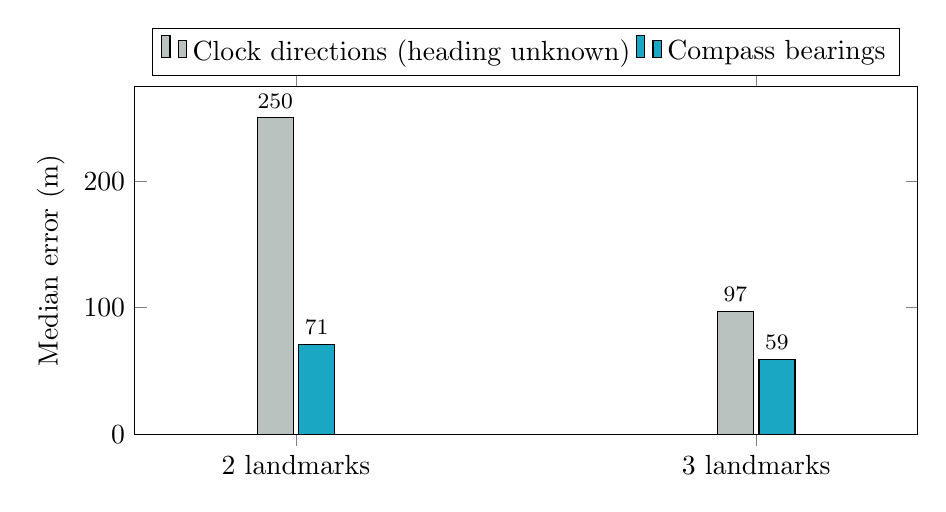
\begin{tikzpicture}
\begin{axis}[ybar, width=0.95\linewidth, height=6cm, bar width=13pt, ymin=0,
  ylabel={Median error (m)}, symbolic x coords={2 landmarks, 3 landmarks},
  xtick=data, legend style={at={(0.5,1.03)},anchor=south,legend columns=-1},
  nodes near coords, enlarge x limits=0.35, every node near coord/.append style={font=\footnotesize}]
\addplot[fill=greyN!60] coordinates {(2 landmarks,250) (3 landmarks,97)};
\addplot[fill=cyanN] coordinates {(2 landmarks,71) (3 landmarks,59)};
\legend{Clock directions (heading unknown), Compass bearings}
\end{axis}
\end{tikzpicture}
\caption{Compass bearings against clock directions, 30 random spots, named landmarks 80--900 m away and more than
35$^\circ$ apart. Within 75 m with 2 landmarks: 57 \% against 13 \%.}\label{fig:compasschart}
\end{figure}

\begin{table}[htbp]\centering\small
\caption{3D line of sight and Aim \& tap, 60 simulated casualties per area at spots where at least one landmark
top is truly in sight. Same spots and random draws in every row (\code{scripts/eval\_geomatics.py --seen}).}\label{tab:geomatics}
\begin{tabular}{lrrrr}
\toprule
& \multicolumn{2}{c}{Streets} & \multicolumn{2}{c}{Woods}\\
\cmidrule(lr){2-3}\cmidrule(lr){4-5}
& median error & within 50 m & median error & within 50 m\\
\midrule
Before (distance + canopy rule) & 417 m & 7 \% & 492 m & 5 \%\\
+ 3D line of sight & 190 m & 23 \% & 427 m & 8 \%\\
+ Aim \& tap (tilt, turn) & \textbf{75 m} & \textbf{45 \%} & 469 m & 10 \%\\
\bottomrule
\end{tabular}
\end{table}

\begin{table}[htbp]\centering\small
\caption{In the woods, 60 simulated casualties in wooded cells, one report then up to 3 questions
(\code{scripts/eval\_forest.py}).}\label{tab:forest}
\begin{tabular}{lrrr}
\toprule
& median error & within 75 m & within 150 m\\
\midrule
Before & 1,123 m & 3 \% & 5 \%\\
+ canopy-aware visibility & 1,155 m & 0 \% & 3 \%\\
+ ``in the woods, dirt track'', ground and traffic questions & 473 m & 10 \% & 23 \%\\
+ phone compass & 458 m & 12 \% & 22 \%\\
\bottomrule
\end{tabular}
\end{table}

\begin{caveat}
\begin{itemize}
  \item In the streets, 57 \% of random spots see \emph{no} landmark top at all, and 73 \% in the woods. There only
        questions and ground or traffic clues remain, and the median error is around 850 m (streets) and 1.5 km
        (woods). Our earlier city numbers assumed landmarks visible whenever close, and were too optimistic.
  \item Canopy-aware visibility doesn't improve the forest numbers by itself; it removes wrong conclusions such as
        ``can't see the keep, so you're far from it''.
  \item The 3D model plays reality in these tests and is also what the localiser uses. Leaves in summer, trucks,
        scaffolding and landmark points placed off the structure will make real results worse.
  \item The map covers the Vincennes sector only. Another area needs its OSM, IGN and LiDAR data fetched.
\end{itemize}
\end{caveat}

\chapter{Asking the right question}\label{ch:questions}

The ask-back loop is what makes Near different, and we never cut it. After each report, Near considers
every question it could ask, predicts how each possible answer would change the position, and asks the one
expected to help most.

\section{Candidate questions}

\begin{table}[htbp]\centering\small
\caption{Question types, the answers modelled, and their effort (load) for the person in the field.}\label{tab:qtypes}
\begin{tabularx}{\linewidth}{lXlc}
\toprule
Kind & Example & Answers & Load\\
\midrule
visible\_type & ``Can you see a railway?'' & yes / no & 1\\
visible\_feature & ``Can you see the Sainte-Chapelle?'' & yes / no & 1\\
which\_see & ``Which of these can you see: the chapel, a tower, the Tour des Salves?'' & any subset & 1.5\\
setting3 & ``Inside, in a street, or in the open?'' & 3 & 1.5\\
hear\_type & ``Have you heard a train in the last few minutes?'' & yes / no & 1\\
ground & ``Under trees? Tarmac, dirt, or no path?'' & 2--3 & 1--1.5\\
left\_right & ``Facing the keep, is the church on your left or right?'' & left / right & 2\\
sun & ``Where is the sun? Give me a clock direction.'' & 12 & 2\\
compass & ``If you have a compass: bearing to the keep? Degrees or mils.'' & 16 sectors or none & 2\\
feature\_dir & ``Where is the Sainte-Chapelle from you? Clock direction.'' & 12 or can't see & 2\\
hear\_dir & ``Where do you hear road traffic from?'' & 12 or none & 2\\
dist\_band & ``Roughly how far is the church, in metres?'' & 5 bands & 2.5\\
describe & ``What landmarks can you see? Clock directions.'' & open & 3\\
\bottomrule
\end{tabularx}
\end{table}

Questions are rebuilt every turn from the current likely spots A/B/C and the real named features around
them. The ``which do you see'' question uses the features whose visibility differs most between the spots.

\section{Choosing one}

For a question $q$ with answers $a$, the answer model gives $P(a \mid p, \theta)$ for every cell and
heading, with realistic noise (a person misjudging left and right, a compass answer in 22.5$^\circ$
sectors, a 40 \% chance of having no compass at hand). With the current posterior $P(p,\theta)$:
\begin{align}
  P(a) &= \sum_{p,\theta} P(a \mid p,\theta)\,P(p,\theta), \\
  P(p,\theta \mid a) &\propto P(a \mid p,\theta)\,P(p,\theta), \\
  \Delta H(q) &= H\big[P(p)\big] - \sum_a P(a)\, H\big[P(p \mid a)\big] \quad\text{(bits)}, \\
  \Delta S(q) &= S\big[P(p)\big] - \sum_a P(a)\, S\big[P(p \mid a)\big] \quad\text{(metres)},
\end{align}
where $S$ is the spread of the position (expected distance to the best guess). Bits alone favour
splitting far-off areas the coordinator doesn't care about; metres alone ignore ambiguity. The score
blends both, then divides by the effort:
\begin{equation}
  \text{score}(q) \;=\; \frac{\text{blend}\big(\Delta H(q), \Delta S(q)\big)}{1 + \lambda\,(\text{load}(q) - 1)} .
\end{equation}

\paragraph{Stopping.} Near stops when the radius is under 75 m, when no question gains at least 0.05 bits,
or when the budget is spent: up to 6 location questions (5 when the speaker sounds stressed, 4 when highly
stressed).

\paragraph{A goal for every question.} The dashboard and the phone show why each question is asked: ``Goal:
tell area A (45 \%) from area B (30 \%) · yes $\rightarrow$ A, no $\rightarrow$ B · error $\sim$600 m $\rightarrow$ $\sim$150 m'',
or ``Goal: a compass bearing removes the unknown facing direction''.

\nanofig{questions}{Choosing a question: each candidate is scored by how much it is expected to shrink the position, given
every answer it could get.}
{Decision-tree infographic, 16:9, plain white background, flat vector. At the top a small map with two
blobs labelled ``A 45\%'' and ``B 30\%''. Below, three candidate question cards side by side: ``Can you see a railway?''
with two branches ``yes'' and ``no'' each showing a tiny map where the blobs change little, score ``0.2 bits'';
``Is the church left or right of the keep?'' with branches ``left'' (only A remains) and ``right'' (only B remains),
score ``0.95 bits, 600 m → 150 m'' highlighted with a cyan glow and a check mark; ``How far is the church?'' with five
small branches, score ``0.4 bits, effort high''. A small label ``asked'' over the winning card. Exactly these labels. Colour palette (use only these): navy \#0D1110, cyan \#1AA7C4, amber \#E09A2B, red \#E5484D, green \#3FA877, grey \#8B9A94, plus white for text on dark shapes.}

\section{Adapting to stress}

\code{stress.py} measures each push-to-talk clip within about 0.3 s of release. It looks at pitch raised
above the speaker's own floor, pitch range (its own numpy pitch tracker, $\pm$2 Hz on test tones),
brightness (1--5 kHz against 50 Hz--1 kHz), articulation rate, choppy speech, and words such as ``hurry'',
``he's dying'', \emph{vite}, repeats and exclamations. The result is low, elevated or high. Shouting over
noise raises pitch and brightness too, so those cues count less when the background is loud. Stress only
changes \emph{how} Near asks. It never touches medical priority.

\begin{table}[htbp]\centering\small
\caption{Question policy by stress level.}\label{tab:stress}
\begin{tabular}{llll}
\toprule
Speaker & Hardest question allowed & Weight $\lambda$ on effort & Wording\\
\midrule
low / unknown & describe everything (3) & 0.10--0.15 & normal\\
elevated & distances (2.5) & 0.35 & normal\\
high & one clock direction or left/right (2) & 0.60 & shortest (``Sun at what o'clock?''), slower read-back\\
\bottomrule
\end{tabular}
\end{table}

\section{Medical questions}

Health questions are asked in MARCH order and don't count against the location budget. Life threats come
first: is the bleeding stopped, is the casualty awake and answering, are they breathing normally, and where
is the wound when an injury has no body part. Then location and health questions take turns: how it
happened, pale, cold or sweaty, how many minutes ago. When the speaker is the casualty, Near says ``you''
(``Has your bleeding stopped?'').

\section{Results}

\begin{table}[htbp]\centering\small
\caption{Question objective, 40 simulated street casualties with 3D line of sight, same spots and draws in every row
(\code{scripts/eval\_questions.py}).}\label{tab:qobj}
\begin{tabular}{lrrr}
\toprule
& Random street spots & \multicolumn{2}{c}{Spots that see a landmark}\\
\cmidrule(lr){3-4}
Objective & median error & median error & within 250 m\\
\midrule
bits only (before) & 735 m & 359 m & 42 \%\\
metres only & 666 m & 344 m & 45 \%\\
\textbf{blend (current)} & 669 m & \textbf{201 m} & \textbf{52 \%}\\
blend, elevated stress & 666 m & 276 m & 50 \%\\
blend, high stress (3 easy questions) & n/a & 617 m & 35 \%\\
\bottomrule
\end{tabular}
\end{table}

Easier questions cost accuracy. Under high stress, the best setting we tested keeps 3 quick questions (617 m);
cutting to 2 gave 791 m. That trade between speed and precision is for the medical mentors to decide.

\chapter{Listening to the place}\label{ch:acoustics}

The microphone records more than words. Every push-to-talk clip also says something about the space around
the phone, and a short chirp at the end of each report measures the distance to the walls. This chapter
describes those clues and how they are matched against the real buildings. It also says honestly how little
they locate on their own.

\section{Four acoustic clues}

\begin{table}[htbp]\centering\small
\caption{Acoustic clues and what they give.}\label{tab:aclues}
\begin{tabularx}{\linewidth}{>{\raggedright}p{3.2cm}>{\raggedright}p{4.6cm}X}
\toprule
Clue & Source & Gives\\
\midrule
Reverberation from the voice & Every push-to-talk clip & Decay time: $\sim$0.1 s outdoors, 0.3--0.6 s small room, 1--5 s hall or church\\
Chirp echo ranging & A 0.5 s sweep (800 Hz--12 kHz) played at the end of each report, or ``Listen 4 s'' & Impulse response: RT60, direct-to-reverberant ratio, the delay of every echo, so the distance to every wall ($d = 343\,\tau/2$)\\
Background level & The operator's own voice as loudness reference (about 76 dB(A) at the phone) & Noise floor in dB(A), $\pm$7 dB, e.g. 58 dB(A) for a residential street\\
Sound scene and sources & YAMNet + AST on the quiet part of the clip, or under the speech at half weight & Inside small / large / outside urban / rural; trains, road traffic, bells, machinery, birds\\
\bottomrule
\end{tabularx}
\end{table}

\nanofig{echo}{Chirp echo ranging in a street: the phone plays a sweep, and each wall returns it after a delay that gives its
distance. One microphone gives distance, never direction.}
{Top-down urban street illustration, 16:9, flat vector, plain white background, buildings as grey blocks with darker roofs.
A soldier with a phone in the middle of a narrow street. Concentric cyan rings radiating from the phone. Two building
facades highlighted, one at 6 m labelled ``echo 6.0 m'' and one across the street at 9 m labelled ``echo 9.0 m'', a
thin label ``street width 15 m (wall-to-wall echo)''. In the corner an inset graph titled ``echogram'' showing a large
first spike labelled ``direct'' and two smaller spikes labelled ``6 m'' and ``9 m'' on a distance axis in metres, with a
shaded band near 1 m labelled ``ground''. Exactly these labels. Colour palette (use only these): navy \#0D1110, cyan \#1AA7C4, amber \#E09A2B, red \#E5484D, green \#3FA877, grey \#8B9A94, plus white for text on dark shapes.}

\section{From audio to clues}

\paragraph{Sound classes.} Two classifiers run side by side on the laptop. YAMNet (Google, 4 MB, CPU) and the
Audio Spectrogram Transformer (AST, 87M parameters, GPU) both output the 521/527 AudioSet classes, grouped into
what matters: rail, traffic, bells, machinery, nature, and the danger groups. Their scores are averaged 0.4/0.6.
Speech windows are removed first; on a voice report, sounds are read under the speech at half weight, and only
what \emph{was} heard counts.

\paragraph{Kind of space.} Reverberation, echoes and scene scores become probabilities over four settings: indoors
small room, indoors large hall, outdoors between buildings, outdoors open ground.

\paragraph{Impulse response.} \code{spatial.py} deconvolves the recorded chirp with the known sweep, finds the direct
sound, and lists the reflections after it. A reflection between 0.8 and 1.8 m is usually the ground or a ceiling
and isn't counted as a wall. In a reverberant room the first wall echo hides in the tail, so it's marked low
confidence and not used.

\section{Matching against the real place}

\code{surround.py} computes what the phone \emph{should} hear at every spot: 9 spots per 25 m cell, 245,520 in
all, cached in about 25 s.
\begin{itemize}
  \item \textbf{Expected echoes.} 36 rays per spot over a 1 m raster of the IGN footprints. A flat wall reflects
        the chirp from the foot of the perpendicular, so the local minima of distance along the rays are the expected
        echo distances. Two facing walls also give a wall-to-wall echo at the street width. Each measured echo is
        matched to the nearest expected one ($\sigma$ = 0.5 m + 5 \%). A false-alarm floor covers cars, trees and
        people. A big wall within 15 m that returned nothing costs a penalty.
  \item \textbf{Expected noise level.} Every OSM road and rail point is a source: 78 dB(A) at 10 m for a motorway, down
        to 65 for a tertiary road. Each falls off as a line source, loses 15 dB behind a building and 25 dB through a
        facade indoors. In the woods there is no loss for the first 20 m of trees, then 0.05 dB/m, capped at 15 dB.
  \item \textbf{Bits per clue.} The dashboard shows how much each clue narrowed the map, and the area still holding 90 \%
        of the probability with audio alone (the ``Audio match'' layer).
\end{itemize}

\section{Results}

\begin{table}[htbp]\centering\small
\caption{Sound classifiers on 85 labelled real recordings (ESC-50), threshold 0.15.}\label{tab:yamnetast}
\begin{tabular}{lrrrrr}
\toprule
Model & Recall & Precision & F1 & Top group right & False location alarms\\
\midrule
YAMNet & 92 \% & 73 \% & 0.81 & 46/50 & 4/35\\
AST & 80 \% & 98 \% & 0.88 & 45/50 & 0/35\\
\textbf{YAMNet + AST} & 92 \% & 87 \% & \textbf{0.89} & \textbf{48/50} & 2/35\\
\bottomrule
\end{tabular}
\end{table}

\begin{itemize}
  \item \textbf{Blind reverberation} from real sounds in rooms of known RT60: 0.6 s $\rightarrow$ 0.59 s,
        1.2 s $\rightarrow$ 1.12 s, 2.4 s $\rightarrow$ 2.14 s. Small rooms are less precise (0.3 s $\rightarrow$ 0.38 s).
  \item \textbf{Echoes} come back within 0.3 m of the true walls on clips simulated from the real buildings; the noise level
        is within about 3 dB of the model.
  \item \textbf{Ask-back loop} (simulated): median error 102 m with landmarks only, 83 m with the space and sound questions,
        62 m with a Listen clip. That last number is an upper bound, since the clip is drawn from our own model.
  \item \textbf{With 3 landmarks and the sun}, one voice clip with its end chirp raises ``best guess within 75 m'' from 12 \%
        to 18 \% and cuts the median error of the best guess from 1,060 m to 810 m.
\end{itemize}

\begin{caveat}
Audio alone narrows the \emph{kind} of spot, not the place. The true spot ranks in the top 6 \% of the map (median) and
audio removes about 0.8 bits. One microphone hears distance, not direction, and echoes repeat all along a uniform
street, so inside a known 300 m area audio alone is only about 1.5$\times$ better than chance. Scores and thresholds
are not calibrated on real recordings yet. Playing a chirp makes noise; it can be turned off, and reverberation from
the voice still works passively.
\end{caveat}

\section{Heart rate from a chest recording}

\code{heart.py} measures the pulse when the phone's microphone is pressed on the casualty's chest for 10 s. It takes the
envelope of the heart-sound band (25--200 Hz) and its autocorrelation, and checks every multiple of each candidate period
so the ``lub-dub'' gap isn't taken for a beat. On synthetic chest recordings, 96 \% of clean ones were within 5 bpm, and
readings flagged reliable were within 5 bpm 92 \% of the time. Noisy ones are marked ``unclear: press firmly, repeat''.
A voice recording does not carry a usable heart rate, so the dashboard only shows a value from a chest recording, with its
age. Bands: slow $<$ 50, normal, fast $>$ 100, shock range $>$ 120, severe $>$ 140 bpm (placeholders for the mentor).

\chapter{The casualty}\label{ch:casualty}

Everything in this chapter is decision support for trained medics. It organises what was reported, keeps
timers and suggests an order. It never diagnoses or prescribes. Every threshold below is a placeholder to
validate with a medical mentor; all of them sit at the top of their module.

\section{MIST card and priority}

\code{casualty.py} keeps one card per casualty in the format medics use for handover:
\textbf{M}echanism (blast, gunshot, fall, vehicle), \textbf{I}njuries in the speaker's own words,
\textbf{S}igns (conscious, breathing, massive bleeding, AVPU), \textbf{T}reatments with times. Follow-up
reports update the same card. ``He is now unconscious'' changes the signs without the word ``casualty''.

Priority is rule-based. A casualty is \emph{urgent} with massive bleeding, a tourniquet, unconsciousness
or a breathing problem; otherwise \emph{priority} or \emph{routine} from what was said. The evacuation order
is: priority, then who gets worse first, then the oldest tourniquet, then distance to the CCP.

\section{Condition and ``worse in'' windows}

\code{condition.py} gives each casualty a MARCH state with what it rests on:
\begin{itemize}
  \item \textbf{M}assive bleeding: not controlled / controlled / tourniquet / control unknown.
  \item \textbf{A}irway: at risk if unresponsive, gurgling, snoring or gasping; open if talking.
  \item \textbf{R}espiration, \textbf{C}irculation (pale, cold, sweaty, thirsty, weak pulse = shock signs),
        \textbf{H}ead and hypothermia.
\end{itemize}
Responsiveness (AVPU) comes from what is said (``confused'', ``only to pain''), from a speaker who is the
casualty (``I'm hit''), or from vocalising heard on the clip. Distress comes from the casualty's own voice,
screams or groans heard, or the buddy's words. Each source can only raise it. The overall state is stable,
serious, critical or very critical (score 0--100).

\begin{table}[htbp]\centering\small
\caption{Threat windows (textbook orders of magnitude, to check with the medical mentor).}\label{tab:windows}
\begin{tabular}{lll}
\toprule
Threat & Window & Counted from\\
\midrule
Massive bleeding not controlled & 3--10 min & injury\\
Airway at risk & 3--5 min & now\\
Breathing problem & 5--30 min & now\\
Shock signs & 15--45 min & now\\
Bleeding, control unknown & 10--30 min & injury\\
Torso or junctional bleeding (no tourniquet possible) & 30--60 min & injury\\
Head injury or blast with reduced consciousness & 30--120 min & injury\\
Hypothermia (November, lying still) & 30--90 min & injury\\
Tourniquet on a limb & 120--360 min & tourniquet time\\
\bottomrule
\end{tabular}
\end{table}

The clock starts at the injury when it's said (``hit 6 minutes ago''), else before the tourniquet, else at the
first report. The read-back names the soonest threat when it's within 15 minutes (``Warning, critical within the
next 4 minutes: massive bleeding not controlled''). Tourniquet timers change colour at 60, 90 and 120 minutes.

\section{Mobility}

\code{mobility.py} gives each casualty one state: can walk, needs help, stretcher, trapped, or unknown.
\begin{itemize}
  \item \textbf{Said first}, in English or French: ``he can walk'', ``il ne peut pas marcher'', ``limping'', ``pinned
        under rubble''. The latest mention wins.
  \item \textbf{Otherwise inferred} and marked as such: unconscious, massive bleeding, breathing problem, a leg
        tourniquet, or a thigh or pelvis wound mean a stretcher. A lower-leg or foot wound means needs help.
        ``Conscious'' with no leg wound means can walk. Anything else is unknown, and a stretcher is planned.
  \item \textbf{Conflicts are flagged}: ``can walk'' said together with a leg tourniquet keeps what was said, shows
        the conflict, and plans the stretcher anyway.
\end{itemize}
Mobility decides between guidance to the CCP and a medic route (Chapter~\ref{ch:routing}).

\section{Body twin, impact graph, kit and team}

\paragraph{Posture} is estimated, never set by hand. Each clue adds points to some postures: what was said
weighs most; unconscious and breathing suggests the recovery position; a chest wound while conscious suggests
sitting up; a leg tourniquet suggests lying on the back. The scores become probabilities shown under a 3D body
(SMPL-X, built locally because its licence forbids redistribution). Injuries go onto the named body segment;
tourniquets are drawn as an orange band with their running time.

\paragraph{Impact graph.} \code{response.py} draws, from left to right: what was reported $\rightarrow$ body
region $\rightarrow$ structures possibly impacted (dashed, to check: thigh bleeding $\rightarrow$ femoral artery;
blast $\rightarrow$ eardrums, blast lung, concussion) $\rightarrow$ MARCH threat $\rightarrow$ what to bring. How it
happened points to where to look: a fall points to the neck, spine and pelvis; a penetrating wound to a possible
exit wound.

\paragraph{Body parts graph.} Body $\rightarrow$ 7 regions $\rightarrow$ 40 parts. Red means affected (said); orange
means no data yet, which is not the same as fine.

\paragraph{Kit and team.} Kit in MARCH order with quantities and who uses it: tourniquets for limb bleeding, packing
only for junctional wounds, chest seals for chest wounds, a pelvic binder for blast with leg wounds. The team is
the smallest that can carry: 4 bearers per stretcher (2 under 100 m, +2 relief beyond 500 m), escorts for walking
wounded, one medic per two urgent casualties, plus extraction tools for a trapped casualty. Every extra person is
one more target for drones.

\nanofig{casualty}{The casualty view: MARCH state with countdowns, the body twin, and the impact graph from what was said to
what to bring.}
{Medical decision-support infographic, 16:9, plain white background, clean flat vector, red, amber, green and grey status
colours. Left: a vertical MARCH strip with five rows ``M Massive bleeding: tourniquet'' (amber), ``A Airway: open''
(green), ``R Breathing: unknown'' (grey), ``C Circulation: shock signs'' (red), ``H Hypothermia risk'' (amber), each
with a small countdown bar; a label ``worse in 4–10 min''. Centre: a neutral grey 3D human body lying on its back,
seen from above at an angle, left thigh glowing red with an orange band labelled ``TQ 14:32 · 72 min''. Right: a
left-to-right graph of rounded boxes ``left leg bleeding'' → ``left thigh'' → ``femoral artery (check)'' (dashed) →
``M · massive bleeding'' → ``tourniquet, packing''. Small footer text ``decision support, not a diagnosis''. No gore.
Exactly these labels. Colour palette (use only these): navy \#0D1110, cyan \#1AA7C4, amber \#E09A2B, red \#E5484D, green \#3FA877, grey \#8B9A94, plus white for text on dark shapes.}

\chapter{Threats: danger zones}\label{ch:danger}

The map shows the threats each unit heard or named, as coloured zones. They also steer the routes in the next
chapter.

\section{Where threats come from}

\paragraph{Said by the soldier.} \code{danger.py} recognises six threat types in English and French: drone,
small-arms fire, sniper, explosions or shelling, armour, mines or IEDs. Negations (``no drones'') and injury
words (``gunshot to the chest'', ``blast'') don't count. A direction is taken from a clock hour, a compass word
(``from the north'', French \emph{est} only after a preposition), a numeric bearing (``sniper, bearing 1600
mils''), or ``overhead''. It can sit in the same clause or the next one (``taking fire, from my 3 o'clock'').

\paragraph{Heard by the microphone.} Gunfire (``Gunshot, gunfire'', ``Machine gun'', ``Fusillade'') and explosions
(``Explosion'', ``Artillery fire'', ``Boom'') come from YAMNet + AST: an alert fires if any 1 s window of YAMNet or
the whole clip in AST scores at least 0.3. Drones need a dedicated model, because AudioSet has no drone class. On
the phone or through a clean microphone we use an AST fine-tuned on drone audio (\code{preszzz} on Hugging Face,
86M parameters). Over the radio we use our own Near-small (Chapter~\ref{ch:models}). Wind on the microphone puts a
``doubtful'' flag on explosion alerts.

\section{From events to zones}

One phone can't locate a shooter or a drone. So each zone is centred on the \emph{reporter's} estimated position.
Its size is the distance at which that threat is usually heard or seen, plus the reporter's own uncertainty.

\begin{table}[htbp]\centering\small
\caption{Threat types (ranges and lifetimes are placeholders for the mentors).}\label{tab:threats}
\begin{tabular}{llrrl}
\toprule
Type & Colour & Range & Fades after & Packet code\\
\midrule
Drone & pink & 150 m & 10 min & U\\
Small-arms fire & red & 400 m & 15 min & G\\
Sniper & orange & 600 m & 30 min & S\\
Explosions / shelling & yellow & 800 m & 30 min & X\\
Armour & purple & 500 m & 20 min & A\\
Mines / IED & brown & 60 m & 24 h & M\\
\bottomrule
\end{tabular}
\end{table}

\begin{itemize}
  \item \textbf{Circle:} radius = position uncertainty + range (``overhead'': + half the range).
  \item \textbf{Wedge:} if a direction is given and the facing direction is known (heading confidence $\geq$ 5, from the
        sun, a compass, or walking direction), the zone becomes a 50$^\circ$ wedge of radius uncertainty + 1.5 $\times$ range.
  \item \textbf{Unplaced:} a reporter located worse than $\pm$500 m gets a ``?'' label instead of an area, and isn't used
        for routing.
  \item \textbf{Likely source area:} where zones from two or more units overlap (product of soft memberships on a 20 m
        grid), a thick ring marks it. It's only kept when the overlap is clearly smaller than the smallest zone.
  \item \textbf{Pinned in place:} a unit that walks away leaves its threats where it reported them.
  \item \textbf{``Near you'':} a unit standing inside another unit's zone is warned in its read-back.
\end{itemize}

\nanofig{danger}{Danger zones on the coordinator map: circles and wedges around reporters, dashed when heard by a microphone,
and a thick ring where two units' reports overlap.}
{Top-down dark tactical map of a small town, 16:9, the map drawn in near-black navy tones as a rounded rectangle on a plain white background, thin grey streets and building blocks.
A translucent red circle with a solid outline labelled ``SMALL-ARMS FIRE · voice'' around a unit marker ``C1''. A
second translucent red circle with a dashed outline labelled ``SMALL-ARMS FIRE · heard'' around unit ``C2''. Where the
two circles overlap, a thick red ring labelled ``likely source area''. A pink dashed circle labelled ``DRONE'' around unit
``C3''. An orange 50-degree wedge labelled ``SNIPER · bearing 1600 mils'' pointing east from unit ``C4''. A small legend
box at bottom right with coloured squares: Drone, Small-arms fire, Sniper, Explosions, Armour, Mines. Exactly these labels. Colour palette (use only these): navy \#0D1110, cyan \#1AA7C4, amber \#E09A2B, red \#E5484D, green \#3FA877, grey \#8B9A94, plus white for text on dark shapes.}

\section{Results on real recordings}

\begin{table}[htbp]\centering\small
\caption{Danger detection on real recordings, laptop models, clean audio (\code{scripts/eval\_danger.py}).}\label{tab:dangereval}
\begin{tabularx}{\linewidth}{Xl}
\toprule
Test & Result\\
\midrule
88 real gunshot recordings (HEAR gunshot triangulation) & small-arms alert on 97 \% (small arms or explosion: 100 \%)\\
150 drone clips (DADS) & drone alert on 72 \% (first evaluation; 91 \% on another 150-clip shard)\\
85 no-danger ESC-50 clips (helicopter, airplane, engine, door knocks, wind...) & false alarm on 2 \% (wind read as explosion, now flagged doubtful)\\
\bottomrule
\end{tabularx}
\end{table}

The drone detector's model card claims 99.6 \%, which we don't reproduce. It may also have been trained on DADS, so
our drone recall is optimistic. The more useful number is zero drone false alarms on helicopters and airplanes.

\chapter{Getting people back: routing and guidance}\label{ch:routing}

Once a casualty is located, two things can happen. If they can walk, Near guides them to the CCP by voice
and moves their pin as they walk. If they can't, Near plans the route for the medic team going out. Both
routes avoid the danger zones.

\section{The walking network}

\code{route.py} builds a graph from every walkable way in the cached OpenStreetMap data: residential streets,
footways, paths and tracks (\code{forest.geojson}), plus primary to tertiary roads (\code{lines.geojson}).
Motorways, trunk roads and tunnels are left out.
\begin{itemize}
  \item Points that share an OSM node have identical coordinates, so ways join there. Points closer than 4 m are
        also joined, which repairs small gaps in the drawing.
  \item Edges longer than 40 m are cut, so the danger check along them stays fine-grained.
  \item Result: 45,565 nodes and 75,768 edges, built in about 1 s. Start and end points snap to the largest
        connected component (44,781 nodes).
\end{itemize}

\section{The cost of a route}

Each edge $e$ of length $\ell_e$ costs
\begin{equation}
  c_e = \ell_e \left(1 + \sum_{z \in \text{zones}} w_{\text{type}(z)} \cdot \text{conf}_z \cdot
  \text{fresh}_z \cdot m_z(e)\right),
\end{equation}
where $m_z(e) \in [0,1]$ is the soft membership of the edge's midpoint in zone $z$ (1 inside, falling to 0 over
15 \% of the radius + 25 m), $\text{fresh}_z = 1 - \text{age}/\text{lifetime}$, and the type weights are
placeholders: mines 200, sniper 40, small arms 30, armour 25, explosions 15, drone 8. A weight of 30 means one
metre under small-arms fire is worth 30 extra metres of walking. Unplaced zones are ignored.

Dijkstra (scipy, sparse matrix) runs twice: once on this cost and once on plain length. The difference is what
the coordinator sees: ``+390 m detour, avoids 398 m inside the small-arms zone'' in the test scene. Each route
takes about 30 ms, and results are cached by start, end and risk map.

\nanofig{routing}{A walking route that bends around a reported small-arms zone, cut into spoken legs with landmark cues.}
{Top-down map illustration, 16:9, plain white background, flat vector, streets in light grey, buildings in pale blocks, a castle
keep icon. A start marker ``casualty'' at bottom-left and a ``CCP'' cross marker at top-right. A thin grey dashed straight-ish
route labelled ``shortest: 732 m'' passing through a translucent red circle labelled ``small-arms fire''. A thick cyan route
labelled ``safest: 1,122 m'' bending around the circle. Along the cyan route, numbered leg markers 1 to 5 at turns, with
small callouts: ``1: keep at your 7 o'clock, 30 m'', ``2: turn left, 40 m'', ``3: turn left, 100 m, keep on your right'',
``4: turn right'', ``5: CCP''. Exactly these labels. Colour palette (use only these): navy \#0D1110, cyan \#1AA7C4, amber \#E09A2B, red \#E5484D, green \#3FA877, grey \#8B9A94, plus white for text on dark shapes.}

\section{Spoken legs}

The route is simplified with Douglas--Peucker at 12 m, so wiggles smaller than that aren't announced as turns.
Nearly straight continuations (under 25$^\circ$) on the same street are merged, and so are legs under 15 m. Each leg
gets:
\begin{itemize}
  \item a turn word: straight on ($<$ 25$^\circ$), bear ($<$ 60$^\circ$), turn ($<$ 150$^\circ$), turn back;
  \item a length rounded for speech (10 m steps below 100 m, then 50 m);
  \item the street name if OSM has one;
  \item a landmark cue at its end: the nearest named landmark within 150 m and its side (left, right, ahead), not
        repeated from the previous leg;
  \item for soldiers who gave compass bearings, the leg's magnetic bearing, in degrees or in mils, matching the unit they used.
\end{itemize}

The first leg can't say ``turn left'', so it's oriented with what the speaker already gave us. That's their own
heading if it's known, otherwise a landmark they reported (``Walk with the Donjon at your 7 o'clock''), otherwise
the sun, otherwise a compass point. When a route changes mid-walk, the new first leg is given relative to the
current walking direction.

\section{Dead reckoning: the pin follows the walker}

The pin moves along the route by distance walked $s$, with an uncertainty radius $r$ that grows from the last
confirmation:
\begin{align}
  s &= s_0 + \begin{cases} 0.7\,\text{m} \times (\text{steps} - \text{steps}_0) & \text{phone step counter}\\
                            v \cdot \Delta t & \text{time only } (v = 1.1 \text{ m/s walking, } 0.6 \text{ assisted})\end{cases}\\
  r &= r_0 + k \cdot (s - s_0), \qquad k = 0.10 \text{ (steps)},\; 0.25 \text{ (time only)}.
\end{align}
\begin{itemize}
  \item With time only, the pin waits at the end of the current leg instead of guessing that the walker turned,
        and after 30 m of overshoot the phone says ``say next when you reach the turn''.
  \item ``Reached'' (button, or ``next'' said on the radio) snaps the pin to the junction and shrinks the radius to
        40 \% of what it was (at least 20 m).
  \item A pace count over the radio (``300 metres done'') sets the distance on the current leg directly.
  \item A new landmark report re-locates the walker around the dead-reckoning position (Chapter~\ref{ch:loc}), and the
        route restarts from there.
  \item ``I'm lost'' stops the guidance and asks for landmarks with clock directions.
\end{itemize}

\nanofig{deadreckoning}{The uncertainty of a walking casualty's position: it grows with distance walked and snaps back at each
confirmed turn.}
{Clean technical chart-style illustration, 16:9, plain white background. A horizontal axis ``distance walked (m)'' and a vertical
axis ``uncertainty radius (m)''. A cyan sawtooth line: rising slopes labelled ``+25\% of distance (time only)'' and a gentler
dashed amber line labelled ``+10\% (step counter)'', dropping sharply at three vertical markers labelled ``reached turn 1'',
``reached turn 2'', ``reached turn 3''. Above the chart, a small top-down strip of a walking route with a moving pin and a circle
that grows and shrinks. Minimal, exact labels only. Colour palette (use only these): navy \#0D1110, cyan \#1AA7C4, amber \#E09A2B, red \#E5484D, green \#3FA877, grey \#8B9A94, plus white for text on dark shapes.}

\section{Rerouting and warnings}

A background loop moves every guided walker every 2 s. When the set of danger zones changes, it checks the
rest of the walker's route.
\begin{itemize}
  \item If more than 20 m of the remaining route now lies inside a zone and a safer route exists, the walker gets
        the new route: ``New danger reported on your way. New route. Turn left, then about 80 metres.''
  \item If there's no safer route, the walker gets a spoken warning instead.
\end{itemize}
Danger zones are pinned where they were reported, so a walking reporter doesn't drag its own threats along.

\section{Medic route for casualties who can't walk}

For stretcher or trapped casualties located within 500 m, the map shows a dashed amber route from the CCP to the
casualty, with time out (1.3 m/s) and time back carrying a stretcher (0.6 m/s). Both speeds are placeholders.
The route uses the same risk-weighted cost, and is shown only once the position is no longer split between
several areas.

\section{Voice commands while walking}

``Next'' or ``reached'', ``repeat'', ``I'm lost'', ``arrived'', ``stop guidance'', in English and French
(\emph{suivant}, \emph{répète}, \emph{perdu}, \emph{arrivé}). A sentence longer than eight words is treated as a
report, not a command. The same commands come from the phone's buttons or, offline, inside a data packet.

\section{Why not reinforcement learning}

We were asked whether reinforcement learning (RL) could find better routes. For the route itself, no. Both the
network and the risk map are known when a route is needed, so the safest route is a shortest-path problem that
Dijkstra solves exactly in 30 ms. RL would learn an approximation of that answer, need a simulator and training,
and give a medic no reason they can check. Sequential decision-making under uncertainty does help in four places.
They're ranked below; the full write-up is in \code{reports/Route planning and reinforcement learning.md}.
\begin{enumerate}
  \item \textbf{The walker doesn't know exactly where he is.} Choose the instruction that works best on average over
        the position probabilities (a POMDP; the QMDP approximation uses a single cost-to-go map computed by one
        Dijkstra run from the CCP). About half a day of work, and our next step.
  \item \textbf{Threats found on the way, or moving.} This is the Canadian Traveller Problem. Our current policy,
        replanning on every new report, is the standard baseline; hedging policies do better.
  \item \textbf{Learning the risk weights} from after-action data with inverse RL. That needs data we don't have.
  \item \textbf{Dispatching several medic teams}, which is where military medical-evacuation research actually uses
        MDPs and RL (approximate dynamic programming, Q-learning).
\end{enumerate}

\begin{keyresult}[Tested (\code{tests/test\_guide.py}, 10 tests)]
Route avoids a small-arms zone placed on the direct path; simulated walker reaches the CCP with each turn confirmed and no
instruction spoken twice; clock-only mode waits at the turn; step counter moves the pin 120--160 m for 200 steps; a sniper
reported across the rest of the route triggers a reroute; voice commands; threats stay where reported; medic route for a
stretcher case; compass bearings in mils and pace count for a soldier without a phone.
\end{keyresult}

\chapter{War conditions: no internet, no GPS, radio only}\label{ch:offline}

In war there is no internet, no GPS and often no phone signal. Near phones sitting near the front are
switched off or in airplane mode, because any emitter can be located. What every unit keeps is the
tactical voice radio. This chapter describes how Near works with nothing else, and how a phone, if one is
available, adds its sensors without a data network.

\section{What runs offline on the laptop}

\begin{table}[htbp]\centering\small
\caption{Every dependency that used to need the internet, and its offline replacement.}\label{tab:offline}
\begin{tabularx}{\linewidth}{>{\raggedright}p{3.4cm}>{\raggedright}p{4.3cm}X}
\toprule
Need & Before (online) & Now (offline)\\
\midrule
Speech-to-text & Chrome recognition (Google servers) & Whisper large-v3-turbo on the GPU, small on CPU; 0.3--0.5 s per transmission\\
Language model & Mistral API & Mistral 7B served locally by Ollama (optional; rules always run)\\
Map background & tile.openstreetmap.org & 682 tiles drawn on the laptop from our own OSM and IGN data (13 s, zooms 13--17)\\
Map and 3D libraries & unpkg CDN & Bundled in \code{frontend/vendor/}\\
Sound models & Hugging Face downloads & Cached once; loaded with \code{local\_files\_only}\\
Spoken replies & Browser voice, default speaker only & Windows SAPI / espeak-ng to WAV, played on the radio's audio output\\
\bottomrule
\end{tabularx}
\end{table}

One command, run while there is still internet, downloads everything (\code{scripts/fetch\_models.py}); a
second draws the map tiles (\code{scripts/render\_tiles.py}). Rendering our own tiles from data we already
hold also respects OpenStreetMap's tile policy, which forbids bulk downloads.

\section{Radio mode}

\nanofig{radiochain}{Radio mode: the laptop listens to the radio, understands each transmission, and answers on it after the
operator approves.}
{Horizontal signal-chain diagram, 16:9, plain white background, flat vector, navy outlines, amber audio waves, cyan data arrows.
Left: a soldier with a handheld radio, a speech bubble ``This is Bravo 2...''. Zig-zag radio waves to a second radio on a
table at the CCP. An audio cable from the radio's speaker to a laptop labelled ``audio in''. Inside a big laptop outline, a row
of boxes: ``Voice activity: cut transmission'' → ``Data tones? decode packet'' → ``Whisper (local)'' → ``Callsign: BRAVO 2''
→ ``Near pipeline'' → ``Reply draft''. Below the row, a small operator icon with a check mark labelled ``approve''. Then
``Offline voice (SAPI)'' → an audio cable labelled ``audio out'' back to the radio's microphone, and radio waves back to the
soldier with a bubble ``Bravo 2, this is CCP. Copy... Over.''. A crossed-out cloud icon labelled ``no internet''. Exact labels. Colour palette (use only these): navy \#0D1110, cyan \#1AA7C4, amber \#E09A2B, red \#E5484D, green \#3FA877, grey \#8B9A94, plus white for text on dark shapes.}

\paragraph{Wiring.} The radio's speaker output goes into the laptop's audio input, and the laptop's audio output into the
radio's microphone. In the browser, the operator picks both devices on the Radio panel. Replies are played with
\code{setSinkId} on the chosen output, so the laptop's own speaker stays free.

\paragraph{Cutting transmissions.} The page tracks the hiss level when nobody talks (slow average of the RMS). A
transmission starts when the level exceeds four times that floor (at least 0.01). It ends after 900 ms of quiet, or after
30 s. Clips shorter than 0.5 s are dropped. While the laptop is transmitting a reply, listening pauses so it doesn't hear
itself.

\paragraph{Understanding one transmission} (\code{radio.py}):
\begin{enumerate}
  \item \textbf{Data tones} are decoded first (next section). A measurement packet becomes the same evidence as a phone's Listen
        clip.
  \item \textbf{Speech} is transcribed by local Whisper. Transcripts that are only noise words are dropped.
  \item \textbf{Callsign.} ``This is Bravo two'', ``ici Charlie 3'', or a bare ``Bravo 2. Left. Over.'' gives \code{BRAVO 2}.
        A known callsign goes to its open report; a new one opens a report. A transmission with no callsign goes to the
        report heard on the radio in the last 15 minutes. Procedure words (``this is'', ``over'', ``out'', ``roger'') are
        stripped before parsing.
  \item \textbf{Threats in the background sound.} The radio carries more than the voice. Gunfire and explosions come from the
        big laptop models; drones from Near-small, which was trained on radio audio (the big drone model fails there:
        Table~\ref{tab:radioeval}). They're flagged ``heard over the radio''.
  \item \textbf{Reply.} ``Bravo 2, this is CCP.'' + the read-back + ``Over.'' (French: \emph{ici poste de secours} ...
        \emph{À vous}). The operator can edit, send or skip. ``Send without asking'' makes it automatic.
\end{enumerate}

\begin{keyresult}[End-to-end test through a simulated analog radio]
A full spoken report was transcribed word for word, including ``tourniquet on at 1432'' and ``a church at bearing 240
degrees'', with callsign \code{BRAVO 2}. A 25-byte packet sent as tones in the same session added a compass heading, the
kind of space, two wall echoes, the noise level, traffic and a drone threat to the same casualty. A drone recording sent over
the radio raised a drone alert (0.99) on the active casualty. A short answer, ``Bravo 2. Left. Over.'', was routed to the
right report.
\end{keyresult}

\section{Data over the voice channel: the modem}

A phone in airplane mode can still make sound. \code{modem.py} and its JavaScript twin \code{modem.js} turn a few bytes
into audio tones that any voice radio carries. Amateur radio's APRS has sent data this way over FM voice radios for decades.

\begin{table}[htbp]\centering\small
\caption{Modem parameters.}\label{tab:modem}
\begin{tabular}{ll}
\toprule
Modulation & binary FSK, continuous phase\\
Tones & 1200 Hz = 1, 2200 Hz = 0 (inside the 300--3400 Hz radio band)\\
Rate & 400 bit/s (integer samples per bit at 8, 16 and 48 kHz)\\
Frame & preamble 0x55 $\times$ 6 $|$ then twice: sync 0x2D 0xD4 $|$ length $|$ payload $|$ CRC-16 (CCITT)\\
Packet of 40 bytes & $\approx$ 2.0 s of tones with two copies (1.1 s with one)\\
Decode time & 3 ms for a 2 s packet (Python)\\
\bottomrule
\end{tabular}
\end{table}

\paragraph{Decoding.} For each tone, the receiver mixes the signal with $e^{-j2\pi f t}$ and takes the magnitude of its sum
over one bit (a sliding Goertzel-style correlator, computed with a cumulative sum). The soft bit is the mark energy minus the
space energy, normalised. Because the receiver doesn't know where a bit starts, it tries 8 phase offsets per bit. It looks
for the 16-bit sync word with at most one bit wrong, and reads the length byte. The length is also inferred from the gap
between two sync words, in case the byte itself was hit. Each candidate payload is checked against its CRC.

\paragraph{Two copies, added up.} Digital radios lose short frames of audio (about 20 ms each) on a bad link. A lost frame
wipes out 8 bits, so a single-copy packet of 1.1 s rarely survives. Each frame is therefore sent twice, and the receiver adds
the two copies' soft bits before deciding. A dropout rarely hits the same bits in both. This is soft-decision diversity
combining. It's simpler than Reed--Solomon coding, and it's easy to mirror byte for byte in the browser.

\begin{figure}[htbp]\centering
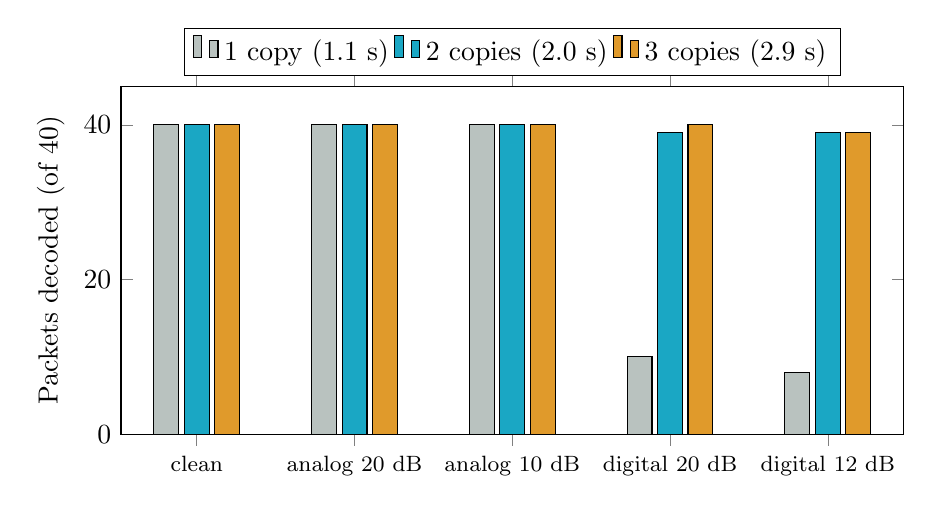
\begin{tikzpicture}
\begin{axis}[ybar, width=0.95\linewidth, height=6cm, bar width=9pt, ymin=0, ymax=45,
  ylabel={Packets decoded (of 40)}, symbolic x coords={clean,analog 20 dB,analog 10 dB,digital 20 dB,digital 12 dB},
  xtick=data, x tick label style={font=\footnotesize}, legend style={at={(0.5,1.03)},anchor=south,legend columns=-1},
  enlarge x limits=0.12]
\addplot[fill=greyN!60] coordinates {(clean,40) (analog 20 dB,40) (analog 10 dB,40) (digital 20 dB,10) (digital 12 dB,8)};
\addplot[fill=cyanN] coordinates {(clean,40) (analog 20 dB,40) (analog 10 dB,40) (digital 20 dB,39) (digital 12 dB,39)};
\addplot[fill=amberN] coordinates {(clean,40) (analog 20 dB,40) (analog 10 dB,40) (digital 20 dB,40) (digital 12 dB,39)};
\legend{1 copy (1.1 s), 2 copies (2.0 s), 3 copies (2.9 s)}
\end{axis}
\end{tikzpicture}
\caption{Random 40-byte packets through the simulated radio channel, random start time and level.}\label{fig:modemchart}
\end{figure}

\nanofig{modem}{The modem: bytes become two audio tones; the frame is sent twice and the two copies are added before deciding
each bit.}
{Technical signal illustration, 16:9, plain white background, flat vector. Top: a row of byte boxes ``55 55 55 55 55 55'' (grey,
labelled ``preamble''), then ``2D D4'' (navy, ``sync''), ``1C'' (``length''), a long cyan block ``payload 28 B'', ``CRC'' (amber),
then the same sync-length-payload-CRC sequence again labelled ``copy 2''. Middle: an audio waveform below the frame alternating
between a lower-frequency sine labelled ``1200 Hz = 1'' and a higher-frequency sine labelled ``2200 Hz = 0''. Bottom: two
rows of soft-bit bars labelled ``copy 1'' and ``copy 2'', each with a short gap labelled ``20 ms dropout'' at different places,
plus a third row labelled ``sum'' with no gap. Exactly these labels. Colour palette (use only these): navy \#0D1110, cyan \#1AA7C4, amber \#E09A2B, red \#E5484D, green \#3FA877, grey \#8B9A94, plus white for text on dark shapes.}

\section{Compact packets}

\code{packet.py} and \code{packet.js} share one byte layout. A packet carries what the phone measured, never raw audio.

\begin{table}[htbp]\centering\small
\caption{Report packet (phone $\rightarrow$ CCP). Fields after the mask are present only if their bit is set.}\label{tab:packet}
\begin{tabularx}{\linewidth}{llX}
\toprule
Bit & Field & Encoding\\
\midrule
-- & type / version & 1 B: 0x11\\
-- & callsign & 1 B length + up to 8 ASCII bytes\\
-- & time and sequence & 2 B: minutes since midnight UTC (11 bits) + sequence (5 bits)\\
-- & field mask & 2 B\\
0 & compass (``12 o'clock'') & 1 B: degrees $\times$ 256 / 360\\
1 & aimed landmarks & 1 B count + 2 B each (azimuth, elevation $\times$ 4)\\
2 & step count & 2 B\\
3 & kind of space & 2 B: 4 probabilities $\times$ 15, 4 bits each\\
4 & noise level & 1 B: dB(A)\\
5 & wall echoes & 1 B count + 1 B each (metres $\times$ 4, 0.25 m steps up to 63.75 m)\\
6 & sounds heard & 1 B count + 1 B each (group 3 bits, score 5 bits)\\
7 & threats heard & 1 B mask (drone, small arms, explosion) + 1 B score each\\
8 & guidance event & 2 B: reached / arrived / lost + leg number\\
9 & strength of the space clues & 1 B\\
\bottomrule
\end{tabularx}
\end{table}

A full measurement packet is 21--35 bytes; the example in Chapter~\ref{ch:eval} carries all ten fields in 32 bytes. The route
packet (CCP $\rightarrow$ phone) is 0x21, callsign, route id, leg count, then 6 bytes per leg: bearing (1 B), length (2 B),
landmark index (2 B, from a list the phone keeps offline) and the side of that landmark (1 B). An 8-leg route is 53 bytes,
about 2.5 s of tones. The same bytes can travel over a radio's data mode or a mesh radio, posted to \code{/api/packet}.

\nanofig{packet}{A 32-byte measurement packet, field by field.}
{Byte-map infographic, 16:9, plain white background, flat vector. A long horizontal strip of 32 small square cells grouped and
coloured by field, with labels above each group: ``type'' (1), ``callsign BRAVO 2'' (8), ``time+seq'' (2), ``mask'' (2),
``compass 75°'' (1), ``aim'' (3), ``steps 1234'' (2), ``space'' (2), ``dB(A) 62'' (1), ``walls 3.5 m, 9 m'' (3), ``traffic''
(2), ``drone 0.85'' (2), ``reached leg 2'' (2), ``strength'' (1). Below the strip, a bracket labelled ``32 bytes = about 2 s of
tones''. Pastel colours per group, navy labels. Exactly these labels. Colour palette (use only these): navy \#0D1110, cyan \#1AA7C4, amber \#E09A2B, red \#E5484D, green \#3FA877, grey \#8B9A94, plus white for text on dark shapes.}

\section{The radio channel we simulate}

\code{radiosim.py} approximates what a radio does to sound, for testing and for training:
\begin{itemize}
  \item \textbf{Analog FM:} band-pass 300--3400 Hz (4th-order Butterworth), automatic gain to a fixed level, soft clipping
        ($\tanh$), resampling to 8 kHz, hiss at 15--30 dB SNR.
  \item \textbf{Digital:} the same, plus 8-bit $\mu$-law quantisation and 3 \% of 20 ms frames lost.
\end{itemize}
Real military radios use speech vocoders (e.g. MELPe) at low bit rates, which model speech and may smear tones and other
sounds further. That's why every radio result in this report needs to be repeated on the unit's actual radio.

\nanofig{radiosim}{The simulated radio channel used for tests and training.}
{Signal-processing block diagram, 16:9, plain white background, flat vector. Left: a clean colourful spectrogram labelled ``phone
microphone''. Then boxes in a row connected by arrows: ``band-pass 300–3400 Hz'', ``automatic gain + soft clipping'',
``8 kHz'', ``8-bit µ-law (digital)'', ``lost 20 ms frames (digital)'', ``hiss 15–30 dB''. Right: the same spectrogram now narrow
in frequency, with two black vertical gaps and grainy noise, labelled ``what the CCP hears''. Exactly these labels. Colour palette (use only these): navy \#0D1110, cyan \#1AA7C4, amber \#E09A2B, red \#E5484D, green \#3FA877, grey \#8B9A94, plus white for text on dark shapes.}

\section{The phone with no network}

If the unit has a phone, it adds sensors the radio can't carry. The field page installs as an offline web app: a service
worker caches the page, the model, the libraries and the landmark list on first load. We tested it by reloading with the
network cut.

\nanofig{phone}{The offline phone: measure, send as tones, receive a route, follow the arrow.}
{Smartphone UI mockup, portrait, dark theme, shown on a plain white background, 9:16 phone inside a 16:9 canvas with
callouts. Screen content top to bottom: header ``NEAR · FIELD'', a card titled ``No network: talk on the radio, send data as
tones'', a text field ``Bravo 2'', a button ``Measure 4 s'', result chips ``outdoors, between buildings 72\%'', ``walls 3.5, 9 m'',
``drone 0.91'', ``62 dB(A)'', a large button ``Send by radio'', two buttons ``Receive route'' and ``Hand-over QR''. Below, a
guidance panel with a big cyan arrow pointing up-right, a chip ``86 m to the next turn'', text ``Leg 2 of 5: bearing 043, about 120
metres. You should see Mairie de Saint-Mandé on your right.'' and a button ``Reached the turn''. Callouts outside the phone:
``runs offline'', ``~30 bytes as 2 s of tones'', ``compass + step counter''. Exactly these labels. Colour palette (use only these): navy \#0D1110, cyan \#1AA7C4, amber \#E09A2B, red \#E5484D, green \#3FA877, grey \#8B9A94, plus white for text on dark shapes.}

\begin{itemize}
  \item \textbf{Measure 4 s.} The phone records 3.1 s of ambient sound, then plays the 0.5 s chirp. Near-small runs in the browser
        (onnxruntime-web, WebAssembly, one thread) and returns threats, sounds and the kind of space. A matched filter on the chirp
        (FFT cross-correlation with the same sweep the phone played) finds the direct sound and up to four wall echoes between
        1.8 and 25 m. The noise level comes from the quiet part, calibrated on the operator's own voice from the last
        push-to-talk (the loudest 20 \% of 50 ms frames taken as about 62 dB(A)).
  \item \textbf{Send by radio.} The operator presses push-to-talk, holds the phone's speaker to the radio's microphone, and
        taps: the packet plays as tones.
  \item \textbf{Receive route.} The phone listens to the radio's speaker, decodes tones every 2.5 s, and starts guiding when
        a route packet arrives. An arrow points along the leg's bearing relative to the compass heading. The step counter
        (accelerometer peaks above the running mean, at least 0.3 s apart, 0.7 m per step) counts down the metres. The turns
        are spoken, with landmark cues from the cached list. ``Reached'' advances the leg and queues a guidance event for
        the next packet.
  \item \textbf{Hand-over QR.} Everything the phone knows (callsign, time, last read-back, threats, facing) as a QR code for the
        medic who arrives.
\end{itemize}

The phone and the laptop were checked against each other in both directions. A packet encoded in JavaScript was decoded
in Python after the simulated digital radio. A route encoded in Python was decoded in JavaScript after the simulated
analog radio.

\section{Soldiers without a phone}

Most of what a phone adds has a spoken equivalent, so a soldier with only a radio loses little:
\begin{itemize}
  \item \textbf{Compass and Aim \& tap $\rightarrow$ spoken compass bearings.} Every soldier carries a compass, and resection
        from bearings is standard land navigation. Two named landmarks give a 71 m median error (Chapter~\ref{ch:loc}).
  \item \textbf{Step counter $\rightarrow$ pace count.} Soldiers are trained to count paces per 100 m; ``300 metres done''
        moves the pin.
  \item \textbf{Phone sound analysis $\rightarrow$ the radio audio itself.} Threats are detected at the CCP in what comes
        through the radio.
  \item \textbf{Echo chirp:} lost. A half-duplex radio can't send a chirp and listen to its echo. The question
        ``indoors, in a street, or in the open?'' partly replaces it.
\end{itemize}

\chapter{Models}\label{ch:models}

Near uses machine-learned models only where rules can't do the job: turning speech into text, recognising
sounds, and filling gaps in odd phrasing. Everything else is explicit, inspectable code: positions, questions,
routes and medical rules. A coordinator can always ask ``why'' and get an answer.

\begin{table}[htbp]\centering\small
\caption{Every model in Near.}\label{tab:models}
\begin{tabularx}{\linewidth}{>{\raggedright}p{3.0cm}>{\raggedright}p{1.3cm}>{\raggedright}p{2.2cm}>{\raggedright}p{2.2cm}X}
\toprule
Model & Size & Licence & Runs on & Used for\\
\midrule
Whisper large-v3-turbo (faster-whisper) & 809M & MIT & laptop GPU, fp16 & Speech-to-text, reports and radio, EN/FR\\
Whisper small & 244M & MIT & laptop CPU, int8 & Same, without a GPU\\
Mistral 7B (Ollama) & 7B & Apache 2.0 & laptop GPU & Optional: fills extraction fields the rules missed\\
YAMNet & 3.7M & Apache 2.0 & laptop CPU & Sound events, scene, gunfire/explosion group scores\\
AST (MIT/ast-finetuned-audioset) & 87M & BSD-3 & laptop GPU & Second sound opinion (0.6 weight); teacher for Near-small\\
Drone AST (preszzz) & 86M & BSD-3 & laptop GPU & Drones in clean audio (phone microphone)\\
CED-tiny (mispeech) & 5.5M & Apache 2.0 & phone (ONNX) & AudioSet classes on the phone, incl. gunfire\\
\textbf{Near-small} (ours) & 5.5M & ours & laptop and phone & Drones over the radio and on the phone; gunfire head\\
SMPL-X body & -- & research licence & laptop (built locally) & 3D casualty twin (not redistributed)\\
\bottomrule
\end{tabularx}
\end{table}

\section{Speech: Whisper}

Whisper is an encoder-decoder transformer trained on a very large amount of weakly labelled multilingual speech \cite{whisper}. The \emph{large-v3-turbo}
variant keeps the large encoder and cuts the decoder to 4 layers, which makes it several times faster with little
loss. We run it through CTranslate2 (faster-whisper) in float16; cuBLAS and cuDNN come from the PyTorch install.
Our settings for radio audio are in Chapter~\ref{ch:language}.

\section{Sounds: YAMNet and AST}

YAMNet is a MobileNet-v1 on 0.96 s log-mel windows that predicts the 521 AudioSet classes. It's small and runs on the
CPU. AST, the Audio Spectrogram Transformer, cuts a 10 s, 128-band log-mel spectrogram into 16 $\times$ 16 patches
and runs a ViT on them. It reaches 0.459 mAP on AudioSet. Their averaged scores (0.4 / 0.6) beat both alone on our
85-recording test (F1 0.89, Table~\ref{tab:yamnetast}).

\section{Near-small: a phone-sized sound model for radio audio}

\paragraph{Why.} The big laptop models were trained on clean recordings, and they collapse when sound goes through a
radio. Over the simulated analog channel the 86M-parameter drone detector caught 9 \% of drones; over the digital
channel, 6 \% (Table~\ref{tab:radioeval}). A phone also can't run 180M parameters. We needed a small model that works
on radio audio and on a phone.

\paragraph{Base.} CED-tiny (Consistent Ensemble Distillation, 5.5M parameters). It's a ViT-style audio transformer
distilled from a large ensemble on AudioSet. It takes 64-band log-mel features (512-point FFT, hop 160 at 16 kHz) and
mean-pools 192-dimensional tokens into the 527 AudioSet outputs. Its label order matches AST's exactly, so AST can teach it
directly.

\paragraph{Architecture.} We keep CED-tiny's encoder and AudioSet head, and add two heads on the pooled features
(LayerNorm + Linear): \emph{drone} and \emph{gunfire}.

\paragraph{Data (never the test clips).}
\begin{itemize}
  \item 3,000 drone clips (DADS shard 4) and 3,000 no-drone clips (DADS shard 0).
  \item 2,000 gunshot and 2,000 forest-background clips from the tropical-forest gunshot set (Katsis et al. 2022, augmented
        release \code{aazmaine25/tropical-gunshot-wda-dataset}). This is a different source from the 88 gunshots we test on.
  \item Random 2 s crops, random gain 0.3--1.5.
\end{itemize}

\paragraph{Training with radio-aware distillation.} For each batch:
\begin{enumerate}
  \item AST (the teacher) hears the \emph{clean} crop and gives its 527 probabilities.
  \item The student hears the same crop after the simulated radio: clean 35 \% of the time, analog 35 \%, digital 30 \%.
  \item Loss = binary cross-entropy of the two heads against the labels + 3 $\times$ binary cross-entropy of the student's
        527 outputs against the teacher's.
\end{enumerate}
The student learns to hear through the radio what the big model hears on clean audio. AdamW, one-cycle schedule, learning
rate $2\cdot10^{-5}$ for the encoder and $10^{-3}$ for the heads, batch 32, 2 epochs (624 steps), about 8 minutes on the
RTX 4060.

\nanofig{distill}{Training Near-small: the big model hears the clean clip, the small one hears it through a simulated radio and
learns to give the same answers, plus drone and gunfire.}
{Machine-learning training diagram, 16:9, plain white background, flat vector. Left: a waveform icon labelled ``clean clip''. It
splits into two paths. Upper path: straight into a large box labelled ``AST teacher, 86M'' outputting a bar chart labelled
``527 AudioSet probabilities''. Lower path: through a box labelled ``simulated radio: band-pass, 8 kHz, µ-law, dropouts'' into a
small box labelled ``Near-small student, 5.5M'' that has three outputs: a bar chart ``527 AudioSet'', a single bar ``drone'', a
single bar ``gunfire''. Between the two bar charts a dashed double arrow labelled ``distillation loss ×3''. From the drone and
gunfire bars, arrows to tags ``labels: DADS'' and ``labels: forest gunshots''. Small footer ``8 minutes on a laptop GPU''.
Exactly these labels. Colour palette (use only these): navy \#0D1110, cyan \#1AA7C4, amber \#E09A2B, red \#E5484D, green \#3FA877, grey \#8B9A94, plus white for text on dark shapes.}

\paragraph{What went wrong first.} The first version trained only on drone data with a distillation weight of 1. On
clean audio it caught 88 \% of drones but only 8 \% of gunshots. The training clips held no gunshots, so the model
learned that gunfire never happens. Version 2 added the gunshot data and the gunfire head, lowered the encoder learning
rate and tripled the distillation weight. With a 0.3 threshold it caught 90--100 \% of gunshots and 97--100 \% of drones,
but raised false alarms on radio audio to 20--25 \%.

\paragraph{Choosing thresholds honestly.} We set the alarm thresholds on \emph{validation} clips only: the gunshot set's own
validation split (150 + 150) and 150 held-out no-drone clips, each passed through clean, analog and digital channels.
At 0.7, validation gave gunfire recall 83--93 \% with 1--5 \% false alarms, and drones 96--98 \% with none. On the
test gunshots, though, the gunfire head dropped to 2--23 \%. It learned tropical-forest gunshots, and those don't
transfer to the test recordings. The final rule raises small-arms fire when the AudioSet gunfire classes pass 0.3
\emph{or} the head passes 0.7.

\paragraph{Who does what.} The measured results decide each model's job:
\begin{itemize}
  \item \textbf{Laptop, audio received over the radio:} gunfire and explosions from the big models (60--67 \%), drones from
        Near-small (100 \%).
  \item \textbf{Phone:} gunfire from plain CED-tiny (58 \% on clean audio), drones from Near-small (91 \%). Both go into one ONNX
        file, about 30 ms per clip on a phone CPU.
\end{itemize}

\paragraph{Export for the phone.} \code{export\_small.py} writes one ONNX graph with the mel spectrogram inside: the STFT
is a 1-D convolution with a fixed windowed DFT basis, then a mel filter bank and dB conversion with a 120 dB floor. The
phone needs no audio code. The in-graph front end matches CED's feature extractor to within $10^{-4}$ dB, and ONNX
output matches PyTorch exactly. Size: 45 MB in float32 with both encoders; an int8 version (12 MB) drifts by up to 0.05,
so we ship float32.

\section{Language: rules first, a local LLM second}

The rule parser handles the common cases instantly and predictably, in two languages. Mistral 7B, served locally by
Ollama, is asked for the same JSON schema when phrasing is unusual. Its answer only fills empty fields, so a model
hallucination can't overwrite a parsed tourniquet time. It isn't called for short answers. If the LLM is slow or down,
the rules alone carry on. A 7B model on an 8 GB GPU takes about 6 s per full report.

\chapter{Evaluation}\label{ch:eval}

\section{How we measured}

We judge every feature with a number, and we wrote down when a number is optimistic. Three kinds of tests:
\begin{itemize}
  \item \textbf{Simulated soldiers on real maps.} A fake soldier stands at a random spot and describes what he would
        see through the 3D model, with realistic noise (clock directions rounded to the hour, missed landmarks,
        compass error). He answers questions truthfully. The localiser never sees the true spot. Each comparison uses
        the same spots and random draws in every row. This tests the reasoning, not the soldier.
  \item \textbf{Real recordings.} Gunshots (88, HEAR gunshot triangulation), drones (DADS), everyday sounds (ESC-50), and
        clips never used in training or threshold tuning.
  \item \textbf{Simulated radio.} The same recordings passed through \code{radiosim.py}.
\end{itemize}
The automated suite has 115 tests (\code{pytest}), covering synthetic scenes, the question loop, the parser, danger
zones, routing and guidance, compass bearings, packets and the modem. All pass.

\section{Positioning}

\begin{table}[htbp]\centering\small
\caption{Positioning results in one place.}\label{tab:posall}
\begin{tabularx}{\linewidth}{Xr}
\toprule
Setting & Median error\\
\midrule
Ask-back loop, spots seeing $\geq$ 2 landmarks, up to 3 questions & \textbf{43 m}\\
2 named landmarks, compass bearings / clock directions & 71 m / 250 m\\
3 named landmarks, compass bearings / clock directions & 59 m / 97 m\\
Streets, $\geq$ 1 landmark top in sight: before / 3D line of sight / + Aim \& tap & 417 / 190 / 75 m\\
Spots that see a landmark, question objective bits / metres / blend & 359 / 344 / 201 m\\
Woods: before / + ground and traffic clues / + phone compass & 1,123 / 473 / 458 m\\
Random street spots, no landmark guaranteed in sight & $\approx$ 850 m\\
\bottomrule
\end{tabularx}
\end{table}

The last line matters most for planning. In the streets of Vincennes, more than half of random spots see no landmark
top at all. There Near falls back on questions, ground clues, sounds and compass bearings, and the error stays in the
hundreds of metres. Getting the speaker to step to a spot with a view, or to give one compass bearing, changes everything.

\section{Sound and threats}

\begin{table}[htbp]\centering\small
\caption{Threat detection over the phone microphone and the simulated radio. Gunshots: 88 real recordings. Drones: 150
clips (DADS shard 20). False alarms: 150 held-out no-drone DADS clips / 85 ESC-50 no-danger clips. Near-small: final
rule and validated thresholds.}\label{tab:radioeval}
\begin{tabular}{llrrr}
\toprule
Channel & System & Gunshots & Drones & False alarms\\
\midrule
phone mic & big laptop models (YAMNet + AST + drone AST, 180M) & 100 \% & 91 \% & 4 \% / 2 \%\\
phone mic & CED-tiny, plain (5.5M) & 58 \% & -- & 1 \% / 0 \%\\
phone mic & Near-small (5.5M) & 8 \% & 91 \% & 2 \% / 0 \%\\
\midrule
analog radio & big laptop models & 60 \% & \textbf{9 \%} & 3 \% / 4 \%\\
analog radio & CED-tiny, plain & 35 \% & -- & 1 \% / 0 \%\\
analog radio & Near-small & 48 \% & \textbf{100 \%} & 1 \% / 1 \%\\
\midrule
digital radio & big laptop models & 67 \% & \textbf{6 \%} & 5 \% / 7 \%\\
digital radio & CED-tiny, plain & 32 \% & -- & 1 \% / 0 \%\\
digital radio & Near-small & 51 \% & \textbf{100 \%} & 1 \% / 2 \%\\
\bottomrule
\end{tabular}
\end{table}

\begin{figure}[htbp]\centering
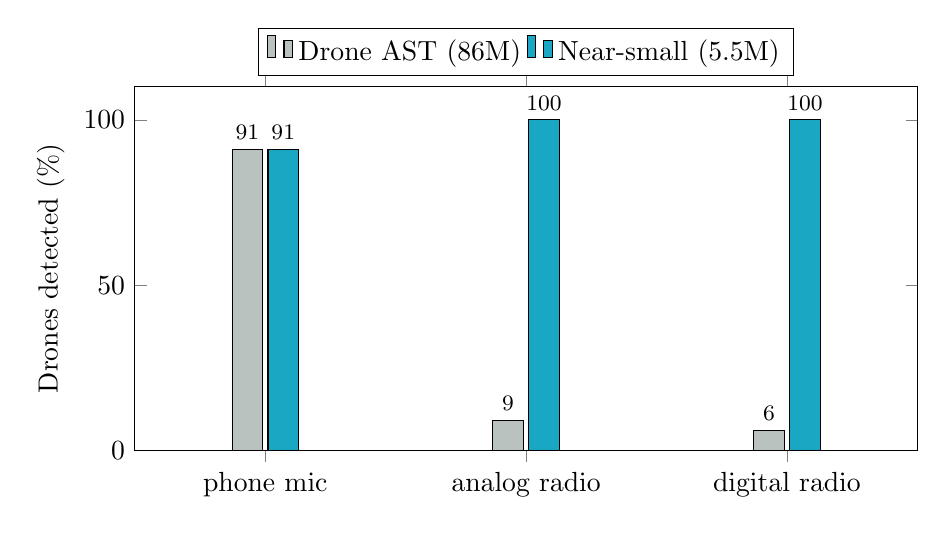
\begin{tikzpicture}
\begin{axis}[ybar, width=0.95\linewidth, height=6.2cm, bar width=11pt, ymin=0, ymax=110,
  ylabel={Drones detected (\%)}, symbolic x coords={phone mic,analog radio,digital radio},
  xtick=data, legend style={at={(0.5,1.03)},anchor=south,legend columns=-1},
  nodes near coords, every node near coord/.append style={font=\footnotesize}, enlarge x limits=0.25]
\addplot[fill=greyN!60] coordinates {(phone mic,91) (analog radio,9) (digital radio,6)};
\addplot[fill=cyanN] coordinates {(phone mic,91) (analog radio,100) (digital radio,100)};
\legend{Drone AST (86M), Near-small (5.5M)}
\end{axis}
\end{tikzpicture}
\caption{Drone detection by channel. The big model collapses when sound passes through a radio; the radio-trained small
model doesn't.}\label{fig:dronechart}
\end{figure}

\begin{caveat}[Read these numbers honestly]
\begin{itemize}
  \item All drone clips come from one dataset (DADS), and the drone AST may have been trained on it. Drone recall on new drones,
        new microphones and real radios will be lower.
  \item The radio channel is our simulation, not a real military radio with a speech vocoder.
  \item Near-small's gunfire head learned tropical-forest gunshots and doesn't transfer well to the test recordings. More varied
        gunshot data is the fix. Until then, gunfire comes from the AudioSet classes of the big models (laptop) and of plain CED-tiny
        (phone).
\end{itemize}
\end{caveat}

\section{Communication}

\begin{itemize}
  \item \textbf{Speech over radio:} a full report and a short answer transcribed word for word through simulated analog and digital
        channels; pure radio hiss gives an empty transcript.
  \item \textbf{Modem:} 40/40 packets on analog radio down to 10 dB SNR; 39/40 on the lossy digital channel with two copies
        (Figure~\ref{fig:modemchart}).
  \item \textbf{Cross-language check:} a 32-byte packet with all ten fields, encoded in JavaScript, decoded in Python after the digital
        channel; an 8-leg route (53 bytes) encoded in Python, decoded in JavaScript after the analog channel.
  \item \textbf{Offline phone:} page reload with the network cut, on-phone model and echo ranging working, no console errors.
\end{itemize}

\section{What we have not tested}

\begin{itemize}
  \item A real walk with GPS off by the Château de Vincennes (the planned demo).
  \item Real tactical radios, especially encrypted digital ones.
  \item Real phones outdoors for the chirp, the step counter and the compass (the browser test used a fake microphone).
  \item Real stressed speakers, and the heart rate on real chests.
  \item Medical thresholds, threat ranges and team sizes with a medical mentor.
\end{itemize}

\chapter{Security, safety and ethics}\label{ch:security}

\section{Emissions are the main risk}

On a modern battlefield, a transmission is a beacon. Near is designed to need few, short transmissions:
\begin{itemize}
  \item one report, then a few questions, each chosen to carry the most information. Every question costs a
        transmission, so we ask the fewest;
  \item measurement packets of about 30 bytes, about 2 s of tones, instead of seconds of raw audio;
  \item a phone that guides offline from one route packet and only transmits at turns or on arrival. The earlier
        connected design polled the server every 3 s, which in the field would be a beacon. It's kept for
        connected use only.
\end{itemize}
In radio mode, Near adds no emitter of its own. The radio the unit already uses carries everything.

\section{Confidentiality and integrity}

\begin{itemize}
  \item \textbf{Nothing leaves the laptop.} Speech-to-text, language model, maps, sound models and voices all run locally. No
        cloud service sees the audio or the positions.
  \item \textbf{Packets are not encrypted yet.} Military radios encrypt the voice channel, and the tones ride inside it.
        On an unencrypted radio, a listener could decode a packet. Authenticated encryption with a pre-shared unit key
        (e.g. AES-CCM, 4--8 bytes of tag) fits the packet budget and is on the roadmap.
  \item \textbf{Spoofing.} A hostile station could send fake reports or packets. Callsign checks, sequence numbers (already in the
        packet), and later authentication tags address this. The coordinator approves every spoken reply.
  \item \textbf{GPS spoofing.} A live GPS fix is just one constraint among many, with an outlier floor. If it disagrees with the
        landmarks, it loses.
\end{itemize}

\section{Medical safety}

Near organises what the field reports. It doesn't diagnose, prescribe or set priorities on its own authority:
\begin{itemize}
  \item every medical rule is a visible, configurable placeholder for medical validation;
  \item ``no data'' is never shown as ``fine'': unknown body parts are orange, unknown MARCH items grey;
  \item inferred values (mobility, posture) are marked as inferred, and conflicts are flagged, not resolved silently;
  \item voice stress changes how questions are asked, never the casualty's priority;
  \item a heart rate is shown only from a chest recording, never estimated from the voice.
\end{itemize}
Depending on use, decision-support software can fall under medical-device rules (in the EU, the MDR). That
classification must be settled before any clinical use.

\section{Dual use and export control}

Near locates and evacuates casualties and maps threats reported by friendly units. It doesn't target anything.
Friendlies only: the design never locates other people, and danger zones mark areas to avoid. Software for military use
may still fall under export-control rules, and any distribution outside the team needs that check.

\section{Failure behaviour}

\begin{itemize}
  \item LLM down $\rightarrow$ rules alone. Sound models missing $\rightarrow$ voice-only positioning. LiDAR missing $\rightarrow$
        building heights and woods.
  \item No position possible $\rightarrow$ ``no position'', never a guess. A town outside the mapped area is detected when named, and
        no position is invented.
  \item Ambiguous position $\rightarrow$ all candidate areas shown and spoken, and no medic route until it's resolved.
\end{itemize}

\chapter{Business case}\label{ch:business}

\section{Value proposition}

\begin{quote}
\emph{Other teams map what you say. We find you when you don't know where you are, by asking the right question.}
\end{quote}

For a military medical chain, Near does three things that save time when time decides who lives:
\begin{itemize}
  \item it gives a position, with an honest radius, for casualties whose reporters can't give one;
  \item it turns a free-form spoken report into a MIST card, timers and an evacuation order without a second person typing;
  \item it plans who goes where, and by which way, around the threats that other units just reported.
\end{itemize}
It does this with what units already carry: a radio, a compass, sometimes a phone, and one laptop at the
collection point.

\nanofig{segments}{Who Near is for: military medical chains first, then civilian rescue where people can't say where they are.}
{Clean business infographic, 16:9, plain white background, flat vector, navy text, cyan and amber accents. A central circle labelled
``Near: locate from what people see''. Around it, five segment cards connected by thin lines: ``Military medical services
(CASEVAC, CCP)'' with a stretcher icon; ``Command posts and training centres'' with a tent and radio icon; ``Ukraine and frontline
partners'' with a radio and drone-crossed icon; ``Emergency call centres (lost callers)'' with a headset icon; ``Mountain rescue and
disaster response'' with a mountain and helicopter icon. Primary segments (first three) in cyan, secondary (last two) in amber, small
legend ``primary'' / ``next''. No flags, no logos. Exactly these labels. Colour palette (use only these): navy \#0D1110, cyan \#1AA7C4, amber \#E09A2B, red \#E5484D, green \#3FA877, grey \#8B9A94, plus white for text on dark shapes.}

\section{Market context}

Analyst estimates vary widely because each firm draws the market's boundaries differently. We quote them only to
show the order of magnitude of the budgets Near plugs into. Our own sizing is bottom-up (next section).

\begin{table}[htbp]\centering\small
\caption{Published market estimates (vendor research, 2025 values).}\label{tab:market}
\begin{tabularx}{\linewidth}{Xrl}
\toprule
Market & 2025 size & Source\\
\midrule
Tactical communication (broad) & USD 26.2 bn, $\sim$7 \%/yr & Fortune Business Insights \cite{fbi-tac}\\
Military tactical radios (narrow) & USD 5.88 bn, 4.6 \%/yr & Fortune Business Insights \cite{fbi-radio}\\
Military medicine (combat casualty care to aeromedical evacuation) & USD 12.5 bn, 6.8 \%/yr & TrendX Insights \cite{milmed}\\
Battlefield medical equipment & USD 8.5 bn, 8.1 \%/yr & SNS Insider \cite{battlemed}\\
\bottomrule
\end{tabularx}
\end{table}

Public money is moving the same way. The European Defence Fund has about €7.3--7.95 bn for 2021--2027, and Ukraine is an
associated country that can join EDF consortia \cite{edf,consilium}. National innovation agencies run defence
programmes for start-ups, among them the French AID, NATO DIANA and Ukraine's Brave1 cluster.

Demand is driven by the two facts in Chapter~\ref{ch:problem}. GPS interference is now routine over Europe (about 123,000
flights affected in four months of 2025 around the Baltic \cite{gps123k}), and drones have stretched evacuation times
from an hour to a day or more \cite{goldenday,wotr}.

\section{Bottom-up sizing method}

We size the opportunity by the number of places where Near would run, not by a share of a vendor estimate:
\begin{equation}
  \text{Revenue} = N_{\text{sites}} \times P_{\text{site}} + N_{\text{areas}} \times P_{\text{area}} + \text{training and support}.
\end{equation}
\begin{itemize}
  \item $N_{\text{sites}}$: casualty collection points, battalion aid stations and command posts that receive casualty reports;
        on the civil side, dispatch centres and rescue bases.
  \item $P_{\text{site}}$: a yearly licence per laptop running Near. Phones and radios add no cost.
  \item $N_{\text{areas}}$, $P_{\text{area}}$: map data packs (landmarks, buildings, LiDAR, paths, tiles, precomputed line of
        sight) per operating area, rebuilt when the area changes.
\end{itemize}
These parameters are hypotheses to test with the first customers; Section~\ref{sec:validate} lists how. We deliberately
give no revenue forecast in this report: a number without a pilot behind it would be made up.

\section{Business model}

\begin{table}[htbp]\centering\small
\caption{Revenue lines (hypotheses to validate).}\label{tab:revenue}
\begin{tabularx}{\linewidth}{>{\raggedright}p{3.6cm}X>{\raggedright\arraybackslash}p{3.6cm}}
\toprule
Line & What the customer gets & Buyer\\
\midrule
Site licence (yearly) & Near on one CCP or command-post laptop, updates, offline models & Military medical service, unit, rescue base\\
Area data pack & An operating area prepared from open and national data: landmarks, buildings, LiDAR line of sight, walking network, offline tiles & Same, per area and refresh\\
Training & Half-day course: spoken bearings, radio procedure with Near, the offline phone & Training centres\\
Integration & Packets and positions into existing systems (battle management, ATAK-type tools), custom radios & Integrators, primes\\
Funded R\&D & Pilots and adaptations paid by defence innovation programmes & EDF consortia, AID, DIANA, Brave1\\
\bottomrule
\end{tabularx}
\end{table}

\section{Why it scales: mass manufacturability}

\begin{itemize}
  \item \textbf{No hardware to build.} Near is software on a commercial laptop. Our demo machine is a gaming laptop with an
        8 GB GPU, and a CPU-only laptop runs it with the smaller Whisper. The field side uses radios and compasses units already
        own; the phone is optional.
  \item \textbf{Near-zero marginal cost.} A new site is a copy of the software and its models (about 2 GB).
  \item \textbf{Areas are built from data, not by hand.} Every area input is open or national data: OpenStreetMap, IGN BD TOPO
        and LiDAR HD in France, Copernicus elevation elsewhere. The scripts fetch and precompute an area in minutes.
  \item \textbf{Robust supply chain.} No custom chips, no proprietary cloud, permissive model licences (MIT, Apache 2.0,
        BSD-3) and our own trained model.
\end{itemize}

\section{Competition}

\begin{table}[htbp]\centering\small
\caption{Competitive landscape.}\label{tab:competition}
\begin{tabularx}{\linewidth}{>{\raggedright}p{3.4cm}XX}
\toprule
Alternative & Strength & Gap Near fills\\
\midrule
ATAK-type situational awareness apps and battle management systems & Standard, widely fielded, rich maps & Positions come from device GPS; no help when the reporter is unsure or jammed\\
MEDEVAC request apps, digital casualty cards & Structured medical data & Need a known location; typing under fire\\
Voice-to-map solutions (other challenge teams) & Fast speech-to-pin, geocoding, trust scores & Assume the speaker can name his position\\
Acoustic gunshot / drone sensors & Accurate source location & Dedicated hardware, fixed sites, cost\\
RF drone detection & Long range & Expensive, emits or needs dedicated sensors; doesn't locate the casualty\\
Manual map and compass resection & Doctrine, no tech & Slow, needs training and calm\\
\bottomrule
\end{tabularx}
\end{table}

\paragraph{What is hard to copy.}
\begin{itemize}
  \item The ask-back loop: choosing the next question by expected error removed, with answer models for 14 question types.
  \item Radio-only operation end to end: callsign routing, local speech, replies approved by an operator.
  \item Data over the voice channel, with packets and a modem built for lossy radios and mirrored in the browser.
  \item A phone-sized sound model trained to hear through a radio. On simulated radio it catches drones that the big model misses.
  \item 3D line of sight from LiDAR, so ``I can't see the keep'' becomes evidence instead of noise.
\end{itemize}
Each piece alone is known technology. The combination, built around a speaker who doesn't know where he is, is ours.

\section{Go-to-market}

\nanofig{gtm}{Go-to-market: from a field trial at Vincennes to funded pilots, then fielding and a civilian version.}
{Horizontal roadmap timeline infographic, 16:9, plain white background, flat vector, navy line with cyan milestones. Four phases
left to right: ``Now: hackathon prototype, Vincennes'' (laptop icon), ``3 months: field trials with a military medical
training unit, real radios'' (radio icon), ``6–12 months: funded pilot (EDF consortium / AID / DIANA), Ukraine partner
trial'' (handshake icon), ``12–24 months: fielded site licences + civilian version for rescue services'' (map and headset
icon). Under the line, small grey labels ``validate'', ``prove'', ``scale''. Exactly these labels. Colour palette (use only these): navy \#0D1110, cyan \#1AA7C4, amber \#E09A2B, red \#E5484D, green \#3FA877, grey \#8B9A94, plus white for text on dark shapes.}

\begin{enumerate}
  \item \textbf{Prove it in the field (0--3 months).} A walk at Vincennes with GPS off; recordings through real tactical
        radios; a session with a military medical training unit to validate the medical rules.
  \item \textbf{Funded pilot (6--12 months).} A pilot with one medical unit or training centre, paid by a defence innovation
        programme; a trial with a Ukrainian partner, where jamming and drones are daily conditions.
  \item \textbf{Fielding (12--24 months).} Site licences and area packs; integration with the battle management system the
        customer already uses.
  \item \textbf{Civilian version.} The same engine for callers who can't give an address (lost hikers, foreign tourists,
        disaster zones without a network). In the EU, network-based caller location is missing in under 3 \% of 112 calls in
        most countries \cite{eu112}, but Advanced Mobile Location needs a SIM and coverage \cite{eu112}. Rescue in
        mountains and disaster areas is where both fail.
\end{enumerate}

\section{How we will validate the business}\label{sec:validate}

\begin{itemize}
  \item \textbf{Need:} interviews with combat medics and CCP coordinators on how often casualty positions are unknown or
        wrong, and how long locating takes today.
  \item \textbf{Fit:} timed exercises, the same scenario with and without Near: time to a usable position, error, number of
        transmissions.
  \item \textbf{Price:} what a medical service pays today for comparable software per site, and how area data is procured.
  \item \textbf{Channel:} whether customers buy directly, through an integrator, or through an innovation programme first.
\end{itemize}

\section{Risks}

\begin{table}[htbp]\centering\small
\caption{Main risks and mitigations.}\label{tab:risks}
\begin{tabularx}{\linewidth}{>{\raggedright}p{4cm}X}
\toprule
Risk & Mitigation\\
\midrule
Real-world accuracy lower than simulated & Field trials before any claim; honest radius; ask-back loop and compass bearings as fallback\\
Radio vocoders garble tones and sounds & Test on target radios; use radio data mode or mesh radio where available; voice-only mode always works\\
Medical-device regulation & Decision-support framing; early regulatory advice; medical validation of every rule\\
Export control and dual-use rules & Early legal check; friendly-forces-only design\\
Long defence sales cycles & Funded pilots, integrators, civilian version in parallel\\
Large incumbents add a similar feature & Speed, the combination of hard pieces, area-pack tooling, field relationships\\
Emissions detected & Few, short transmissions; offline phone; no extra emitter\\
\bottomrule
\end{tabularx}
\end{table}

\section{Team and ask}

\paragraph{Team Fricassé.} Taher Ayadi (pipeline, audio, radio and offline modes, models) and Aziz Maatoug
(geometry, localisation, 3D line of sight, casualty model). We built Near in one weekend at EDTH Paris.

\paragraph{Ask.}
\begin{itemize}
  \item Access to real tactical radios and a military medical training unit for a field trial.
  \item A medical mentor to validate thresholds, windows and team rules.
  \item Introductions to integrators and to defence innovation programmes for a funded pilot.
\end{itemize}

\chapter{Roadmap}\label{ch:roadmap}

\section{Field validation first}

\begin{table}[htbp]\centering\small
\caption{Tests before anyone relies on Near.}\label{tab:fieldtests}
\begin{tabularx}{\linewidth}{>{\raggedright}p{4.2cm}X}
\toprule
Test & What it settles\\
\midrule
Walk at the Château de Vincennes, GPS off & Real positioning error, real question answers, the demo video\\
Aim at the keep from 3--4 surveyed spots & Tilt and turn accuracy against the LiDAR model\\
Recordings through the unit's real radio & Speech, threat sounds and the modem through a real vocoder\\
Phones outdoors & Chirp echoes, step counter, compass, noise calibration\\
Walk in the Bois & The 100 m visibility through trees, noise attenuation, compass under canopy\\
Calm and stressed speakers & Stress levels and the question policy\\
Medical mentor review & Every window, threshold, kit and team rule\\
\bottomrule
\end{tabularx}
\end{table}

\section{Next engineering steps}

\begin{enumerate}
  \item \textbf{Planning over the position uncertainty} (QMDP): choose instructions that work wherever the walker might be. About half a day.
  \item \textbf{Packet authentication and encryption} with a unit key, within the 30-byte budget.
  \item \textbf{More varied gunshot data} for Near-small's gunfire head; drone data from other sources than DADS; training on recordings
        through real radios.
  \item \textbf{Hedged rerouting} for threats discovered on the way (Canadian Traveller policies), and lower drone risk under tree cover.
  \item \textbf{Radio data mode and mesh radio adapters} for the same packets.
  \item \textbf{Area pack tooling}: one command to prepare a new area from open data, outside France too (OSM + Copernicus DEM).
  \item \textbf{Several medic teams}: dispatching across many casualties, where MDP and RL methods are the right tool.
  \item \textbf{Integration} with battle management systems and ATAK-type tools: positions and MIST cards out, reports in.
\end{enumerate}

\appendix
\chapter{API reference}\label{app:api}

\begin{longtable}{>{\ttfamily\raggedright}p{6.2cm}p{8.6cm}}
\caption{HTTP and WebSocket interface of the Near server.}\label{tab:api}\\
\toprule
\normalfont Route & Purpose\\
\midrule
\endfirsthead
\toprule
\normalfont Route & Purpose\\
\midrule
\endhead
GET /map, /field, /pipeline & Coordinator dashboard, field page, step-by-step demo view\\
GET /sw.js & Offline cache (service worker) for the field page\\
POST /api/report & A spoken or typed report or answer (text, optional compass, aims, last fix, voice features)\\
POST /api/transcribe & Audio $\rightarrow$ text with local Whisper\\
POST /api/audio & A Listen clip or the audio of a voice report $\rightarrow$ sound, space, echoes, threats\\
POST /api/voice\_quick & Fast voice features of a push-to-talk clip (stress)\\
POST /api/pulse & Heart rate from a chest recording\\
POST /api/radio & One radio transmission: data tones, speech, threats, callsign $\rightarrow$ report and reply\\
POST /api/packet & A measurement packet from a data link (hex)\\
POST /api/tts & Offline speech (WAV) for a reply, played on the radio's output\\
GET /api/report/\{id\}/guide & Current guidance instruction and progress (phone polling, connected mode)\\
POST /api/report/\{id\}/guide & start, reached, lost, repeat, arrived, stop, steps\\
GET /api/report/\{id\}/route\_tones.wav & The walking route as data tones for an offline phone\\
GET /api/cues & Named landmarks used in route legs, by index (kept offline by the phone)\\
GET /api/report/\{id\}/surround & Measured vs expected surroundings, candidate areas, bits per clue\\
GET /api/report/\{id\}/viz & Spectrogram, sound timeline, echogram of the latest clip\\
GET /api/report/\{id\}/body & Casualty twin: posture, injuries on body segments, tourniquets\\
GET /api/report/\{id\}/response & Impact graph, kit, team\\
POST /api/report/\{id\}/evacuated & Toggle evacuated\\
POST /api/report/\{id\}/auto\_answer & Rehearsal: the simulated soldier answers the pending question\\
POST /api/report/\{id\}/simulate\_listen & Rehearsal: a simulated Listen clip at the true spot\\
POST /api/report/\{id\}/simulate\_pulse & Rehearsal: a simulated chest recording\\
POST /api/simulate & Rehearsal: a simulated soldier at a map point (walking or stretcher case)\\
GET /api/state & Full state (same as the WebSocket)\\
GET /api/landmarks, /api/probe, /api/config & Map landmarks; chirp parameters; offline speech-to-text available\\
POST /api/ccp, /api/reset & Move the collection point; clear everything\\
WS /ws & Full state pushed after every change\\
\bottomrule
\end{longtable}

\chapter{Main parameters}\label{app:params}

All in \code{backend/config.py}. Most are starting points, to tune on real data or validate with a mentor.

\begin{table}[htbp]\centering\small
\caption{Key parameters.}\label{tab:params}
\begin{tabularx}{\linewidth}{>{\ttfamily}lrX}
\toprule
\normalfont Name & Value & Meaning\\
\midrule
CELL\_M, HEADING\_STEP & 25 m, 5$^\circ$ & Grid resolution\\
SIGMA\_CLOCK / RELATIVE / BEARING & 15 / 35 / 6$^\circ$ & Noise of a clock direction, a left/right word, a compass bearing\\
SIGMA\_COMPASS & 25$^\circ$ & Phone compass held still\\
MAG\_DECLINATION & +2$^\circ$ & Magnetic to true north, Paris area\\
OUTLIER\_FLOOR & 0.01 & Any observation can be wrong\\
ACOUSTIC\_WEIGHT & 0.7 & Machine-heard evidence is tempered\\
TARGET\_RADIUS\_M & 75 m & Stop asking below this radius\\
MAX\_QUESTIONS & 6 & Location questions per report (fewer under stress)\\
WALK\_M\_PER\_S & 1.4 & Walking range since the last GPS fix\\
TOURNIQUET\_WARN\_MIN & 60/90/120 & Tourniquet timer colours\\
DANGER\_SOUND\_MIN & 0.3 & Gunfire / explosion alert, laptop models\\
DRONE\_MIN & 0.5 & Drone alert, drone AST\\
SMALL\_GUN\_MIN, SMALL\_DRONE\_MIN & 0.7, 0.7 & Near-small heads, set on validation clips\\
ROUTE\_RISK & 200/40/30/25/15/8 & Mines / sniper / small arms / armour / explosions / drone\\
GUIDE\_START\_R, DISPATCH\_MAX\_R & 200 m, 500 m & Guide a walker / plan a medic route below this radius\\
WALK\_SPEED & 1.1 / 0.6 m/s & Walking, assisted\\
MEDIC\_SPEED, LITTER\_SPEED & 1.3 / 0.6 m/s & Team going out, carrying back\\
STEP\_M & 0.7 m & Step length\\
DRIFT\_STEPS / DRIFT\_TIME & 10 / 25 \% & Position error growth per metre walked\\
\bottomrule
\end{tabularx}
\end{table}

\chapter{Data, models and licences}\label{app:data}

\begin{itemize}
  \item Landmarks, roads, paths, woods: \textcopyright{} OpenStreetMap contributors (ODbL).
  \item Building footprints and heights: IGN BD TOPO; terrain and surface models: IGN LiDAR HD (Licence Ouverte / Etalab 2.0).
  \item YAMNet: Google, Apache 2.0. AST: MIT, BSD-3. Drone AST: \code{preszzz/drone-audio-detection-05-17-trial-0}, BSD-3.
        CED-tiny: \code{mispeech/ced-tiny}, Apache 2.0. Whisper: OpenAI, MIT (faster-whisper / CTranslate2 conversion).
        Mistral 7B: Apache 2.0.
  \item Training and evaluation data (not redistributed): DADS drone audio (MIT); tropical-forest gunshots (Katsis et al. 2022,
        augmented release); HEAR gunshot triangulation; ESC-50 (CC BY-NC 3.0).
  \item SMPL-X body model: research licence, built locally, never committed.
\end{itemize}

\chapter{How to run}\label{app:run}

\begin{lstlisting}
pip install -r requirements.txt
python -m scripts.fetch_models      # once, with internet: Whisper, sound models
python -m scripts.render_tiles      # offline map tiles (13 s)
python run.py                        # http://localhost:8000/map
python run.py --https                # phones on the same network: https://<laptop-ip>:8443/field
python -m pytest -q                  # 115 tests
python -m scripts.eval_radio         # threat detection, phone mic vs simulated radio
python -m scripts.train_small        # retrain Near-small (~8 min on an RTX 4060)
python -m scripts.export_small       # ONNX for the phone
\end{lstlisting}

\chapter{Illustrations}\label{app:prompts}

The illustrations in this report were generated with Nano Banana from the prompts in \code{report/figure\_prompts.md},
then cut out of their white background. They explain ideas; they are not screenshots or measurements. Charts and tables of
results are drawn from the measured numbers, not generated. To replace an illustration, save the new image as
\code{report/figures/<name>.png} and rebuild; if a file is missing, its prompt box is shown instead.

\begin{thebibliography}{99}
\addcontentsline{toc}{chapter}{References}

\bibitem{gps123k} Travel Tomorrow, ``Russian GPS interference disrupts nearly 123,000 flights in four months'', 2025.
\url{https://traveltomorrow.com/russian-gps-interference-disrupts-nearly-123000-flights-in-four-months/}

\bibitem{trtgps} TRT World, reporting on GPS interference in the Baltic region, 2025.
\url{https://www.trtworld.com/world/article/f587da45f7ba}

\bibitem{goldenday} ``A NATO-Russia war would be bloodier than Ukraine, where `golden hour' is already gone, officer says'',
Business Insider via AOL, 2025. \url{https://www.aol.com/articles/nato-russia-war-bloodier-ukraine-132001814.html}

\bibitem{wotr} ``Conflict, CASEVAC, and the golden hour in the age of persistent surveillance'', War on the Rocks, May 2026.
\url{https://warontherocks.com/2026/05/conflict-casevac-and-the-golden-hour-in-the-age-of-persistent-surveillance/}

\bibitem{daylight} ``Ukrainian medic says they `rarely' evacuate wounded soldiers during the day to avoid Russian drone strikes'',
Yahoo News, 2025. \url{https://ca.news.yahoo.com/ukrainian-medic-says-rarely-evacuate-165212780.html}

\bibitem{dignitas} Dignitas Fund, ``When the golden hour disappears: how drone warfare is reshaping battlefield medicine in Ukraine''.
\url{https://dignitas.fund/blog/when-the-golden-hour-disappears-how-drone-warfare-is-reshaping-battlefield-medicine-in-ukraine/}

\bibitem{aspi} ASPI The Strategist, ``Ground robots are transforming battle-casualty evacuation in Ukraine''.
\url{https://www.aspistrategist.org.au/ground-robots-are-transforming-battle-casualty-evacuation-in-ukraine/}

\bibitem{fbi-tac} Fortune Business Insights, ``Tactical Communication Market''.
\url{https://www.fortunebusinessinsights.com/tactical-communication-market-114608}

\bibitem{fbi-radio} Fortune Business Insights, ``Military Tactical Radio Market''.
\url{https://www.fortunebusinessinsights.com/military-tactical-radio-market-118135}

\bibitem{milmed} TrendX Insights, ``Military Medicine Market''.
\url{https://trendxinsights.com/syndicated-market-research-reports/military-medicine-market/}

\bibitem{battlemed} SNS Insider, ``Battlefield Medical Equipment Market''.
\url{https://www.snsinsider.com/reports/battlefield-medical-equipment-market-9880}

\bibitem{edf} European Commission, ``European Defence Fund''.
\url{https://commission.europa.eu/funding-and-tenders/find-funding/eu-funding-programmes/european-defence-fund_en}

\bibitem{consilium} Council of the EU, ``Defence funding''. \url{https://www.consilium.europa.eu/en/policies/defence-funding}

\bibitem{eu112} European Commission, ``2024 report on the implementation of the EU emergency number 112''.
\url{https://digital-strategy.ec.europa.eu/en/library/2024-report-implementation-eu-emergency-number-112}

\bibitem{whisper} A. Radford et al., ``Robust Speech Recognition via Large-Scale Weak Supervision'', 2022.

\bibitem{ast} Y. Gong, Y.-A. Chung, J. Glass, ``AST: Audio Spectrogram Transformer'', Interspeech 2021.

\bibitem{ced} H. Dinkel et al., ``CED: Consistent ensemble distillation for audio tagging'', 2023. \url{https://huggingface.co/mispeech/ced-tiny}

\bibitem{yamnet} Google, YAMNet audio event classifier (AudioSet). \url{https://tfhub.dev/google/yamnet/1}

\bibitem{dads} G. Basso, DADS: Drone Audio Detection Samples. \url{https://huggingface.co/datasets/geronimobasso/drone-audio-detection-samples}

\bibitem{katsis} L. K. D. Katsis et al., ``Automated detection of gunshots in tropical forests using convolutional neural networks'',
Ecological Indicators, 2022. Augmented release: \url{https://huggingface.co/datasets/aazmaine25/tropical-gunshot-wda-dataset}

\bibitem{esc50} K. J. Piczak, ``ESC: Dataset for Environmental Sound Classification'', ACM MM 2015.

\bibitem{qmdp} P. Karkus, D. Hsu, W. S. Lee, ``QMDP-Net: Deep Learning for Planning under Partial Observability'', NeurIPS 2017.

\bibitem{ctp} C. H. Papadimitriou, M. Yannakakis, ``Shortest paths without a map'', 1991 (the Canadian Traveller Problem).

\bibitem{jenkins} P. R. Jenkins, ``Strategic location and dispatch management of assets in a military medical evacuation enterprise'',
AFIT dissertation. \url{https://apps.dtic.mil/sti/pdfs/AD1079716.pdf}

\end{thebibliography}
\nocite{*}


\end{document}
